\documentclass[11pt]{extarticle}
\usepackage{graphicx}
\usepackage{microtype}
\usepackage{float}
\usepackage{amsmath}
\usepackage{amsthm}
\usepackage{amsfonts}
\usepackage{amssymb}
\usepackage{enumerate}
\usepackage{enumitem}
\usepackage{fancyhdr}
\usepackage{mdframed}
\usepackage{multicol}
\usepackage{mathtools}
\usepackage{listings}
\usepackage{verbatim}
\usepackage{tikz}
\usepackage{titling}
\usepackage{bm}
\usepackage{booktabs}
\usepackage{hyperref}
\usepackage{indentfirst}
\usepackage{caption}
\usepackage{titlesec}
\usepackage{xcolor}
\usepackage{tabularx}
\definecolor{uchicagomaroon}{RGB}{128,0,0}
\hypersetup{colorlinks=true, linkcolor=uchicagomaroon, urlcolor=uchicagomaroon, citecolor=uchicagomaroon}
\usepackage[letterpaper, margin=0.62in]{geometry}
\linespread{1.0}

% Tight float spacing
\setlength{\textfloatsep}{3pt plus 1pt minus 2pt}
\setlength{\floatsep}{2pt plus 1pt minus 1pt}
\setlength{\intextsep}{3pt plus 1pt minus 2pt}
\setlength{\abovecaptionskip}{2pt}
\setlength{\belowcaptionskip}{0pt}

% Tight caption
\captionsetup{skip=2pt, font=small, labelfont=bf}

% Compact sections
\titleformat{\section}{\large\bfseries\color{uchicagomaroon}}{\thesection}{1em}{}[\vspace{1pt}\color{uchicagomaroon}\titlerule]
\titleformat{\subsection}{\normalsize\bfseries\color{uchicagomaroon}}{\thesubsection}{1em}{}
\titlespacing*{\section}{0pt}{5pt plus 2pt minus 2pt}{2pt plus 1pt}
\titlespacing*{\subsection}{0pt}{3pt plus 2pt minus 2pt}{1pt plus 1pt}

% Header / footer
\pagestyle{fancy}
\fancyhf{}
\fancyhead[L]{\small\itshape Machine Learning in NBA Over/Under Betting}
\fancyhead[R]{\small Page \thepage}
\fancyfoot[C]{\small Business 35137 $|$ Chicago Booth $|$ Winter 2026}
\renewcommand{\headrulewidth}{0.4pt}
\renewcommand{\footrulewidth}{0.4pt}

% Tighter paragraph spacing
\setlength{\parskip}{1.5pt plus 1pt minus 1pt}
\setlength{\parindent}{1em}

\newcommand{\NN}{\mathbb{N}}
\newcommand{\ZZ}{\mathbb{Z}}
\newcommand{\RR}{\mathbb{R}}
\newcommand{\CC}{\mathbb{C}}
\newcommand{\QQ}{\mathbb{Q}}
\newcommand{\FF}{\mathbb{F}}
\newcommand{\PP}{\mathbb{P}}
\newcommand{\one}{\mathbb{1}}
\newcommand{\LL}{\mathcal{L}}
\newcommand{\JJ}{\mathcal{J}}
\newcommand\norm[1]{\lVert#1\rVert}
\newcommand\set[1]{\left\lbrace #1 \right\rbrace}
\newcommand{\dist}{\operatorname{dist}}
\newcommand{\nt}{\operatorname{int}}
\newcommand{\mean}{\operatorname{Mean}}
\newcommand{\vol}{\operatorname{vol}}
\newcommand{\dpartial}[2]{\frac{\partial #1}{\partial #2}}
\newcommand\independent{\protect\mathpalette{\protect\independenT}{\perp}}
\newcommand{\indep}{\perp \!\!\! \perp}

\title{Final Project Paper}
\author{Alan Donnelly}
\date{March 2026}

\begin{document}

\begin{titlepage}
    \centering
    \vspace*{\fill}
    \small
    {\LARGE \textbf{Machine Learning in Efficient Markets:\\ NBA Over/Under Betting}} \\[2cm]
    {
        Alan Donnelly \\
        Master's in Financial Mathematics \\[0.5cm]
        Andrew McLaughlin \\
        Master's in Financial Mathematics \\[0.5cm]
        Robert Asgeirsson \\
        Master's in Financial Mathematics \\[0.5cm]
        Chris Mulligan \\
        Master's in Financial Mathematics
    } \\[2cm]
    \IfFileExists{University Logo_1Color_Maroon_RGB.png}{%
        \includegraphics[width=0.5\textwidth]{University Logo_1Color_Maroon_RGB.png} \\[0.5cm]
    }{}
    {\large Business 35137: Machine Learning in Finance} \\[0.5cm]
    {\large The University of Chicago Booth School of Business} \\[0.5cm]
    {\large Winter 2026}
    \vspace*{\fill}
\end{titlepage}

\newpage
\tableofcontents

\newpage

%% =====================================================================
%%  SECTION 1: INTRODUCTION
%% =====================================================================
\section{Introduction}

\textbf{Research question.} Can machine learning models---spanning regularised linear methods, dimension reduction, tree-based ensembles, and kernel methods---find exploitable inefficiencies in the NBA over/under betting market, where the Vegas line serves as a near-optimal benchmark? If so, under what conditions can selective betting strategies overcome the sportsbook's commission and generate positive returns?

In sports betting, a \emph{total} (over/under) is the sportsbook's prediction of the combined points scored by both teams. Bettors wager on whether the actual combined score will be over or under this number. Standard odds of $-110$ mean a bettor must risk \$110 to win \$100, implying the sportsbook takes a commission (the \emph{vig}) on every bet. To break even, a bettor must win at least $52.4\%$ of bets---the critical threshold throughout this report.

The Vegas line is set by professional oddsmakers who incorporate team statistics, injuries, matchup history, public betting patterns, and proprietary models. It plays a role analogous to a market price under the efficient market hypothesis (EMH): any model that claims to beat it must find a small, repeatable edge that this well-resourced market process has overlooked---the equivalent of generating alpha in financial markets. This report investigates whether such an edge exists, and directly confronts the gap between statistical significance and economic viability that defines applied machine learning in efficient markets.

A central question in applied machine learning is whether models can reliably outperform an informed benchmark---and if so, whether that statistical advantage translates into economic profit after transaction costs. Sports betting strips away the complications that make financial markets difficult to study cleanly: outcomes are unambiguous (the total is either over or under), payoffs are binary, and the market-maker's edge is precisely quantifiable. The NBA over/under market, with over \$100 billion in annual global sports betting handle, provides an ideal laboratory. We train six model classes using walk-forward validation on 11 NBA seasons (2013/14 through 2023/24), then test the prospectively nominated strategy on a held-out 2024/25 season that was never used in any modelling decision.

\subsection{Approach}
We construct lagged, within-season team features from box score statistics to avoid lookahead bias. Six model classes spanning four families---regularised linear (Ridge, Lasso, ElasticNet), dimension-reduced (PCR), tree-based (XGBoost), and kernel-based (RBF+Ridge)---are evaluated via walk-forward backtesting with strict temporal ordering, tuned on \emph{betting accuracy} rather than regression error, and subjected to Bonferroni-corrected significance tests and block bootstrap confidence intervals. Selective betting with confidence thresholds concentrates bets where the model's edge is strongest. Bankroll simulations with 10 sizing rules---including the Kelly criterion---stress-test whether statistical edge translates into economic viability, and real-world frictions are discussed qualitatively.

%% =====================================================================
%%  SECTION 2: DATA
%% =====================================================================
\section{Data}
Two primary data sources cover 18 NBA seasons (2007/08 through 2024/25). Betting data contains approximately 22,700 games with the Vegas total line, point spread, and final score. NBA box score data provides team-level statistics: points, field goal percentage, three-point percentage, free throw percentage, rebounds, assists, steals, blocks, turnovers, and personal fouls. The two sources are merged on date and team matchup, with team abbreviations standardised for franchise relocations (e.g., NJN $\to$ BKN, SEA $\to$ OKC). The 2024/25 season (1,293 games) is held out entirely; the remaining ${\sim}$21,400 games form the walk-forward pool. COVID-era games are retained with a binary indicator feature.

\begin{figure}[H]
    \centering
    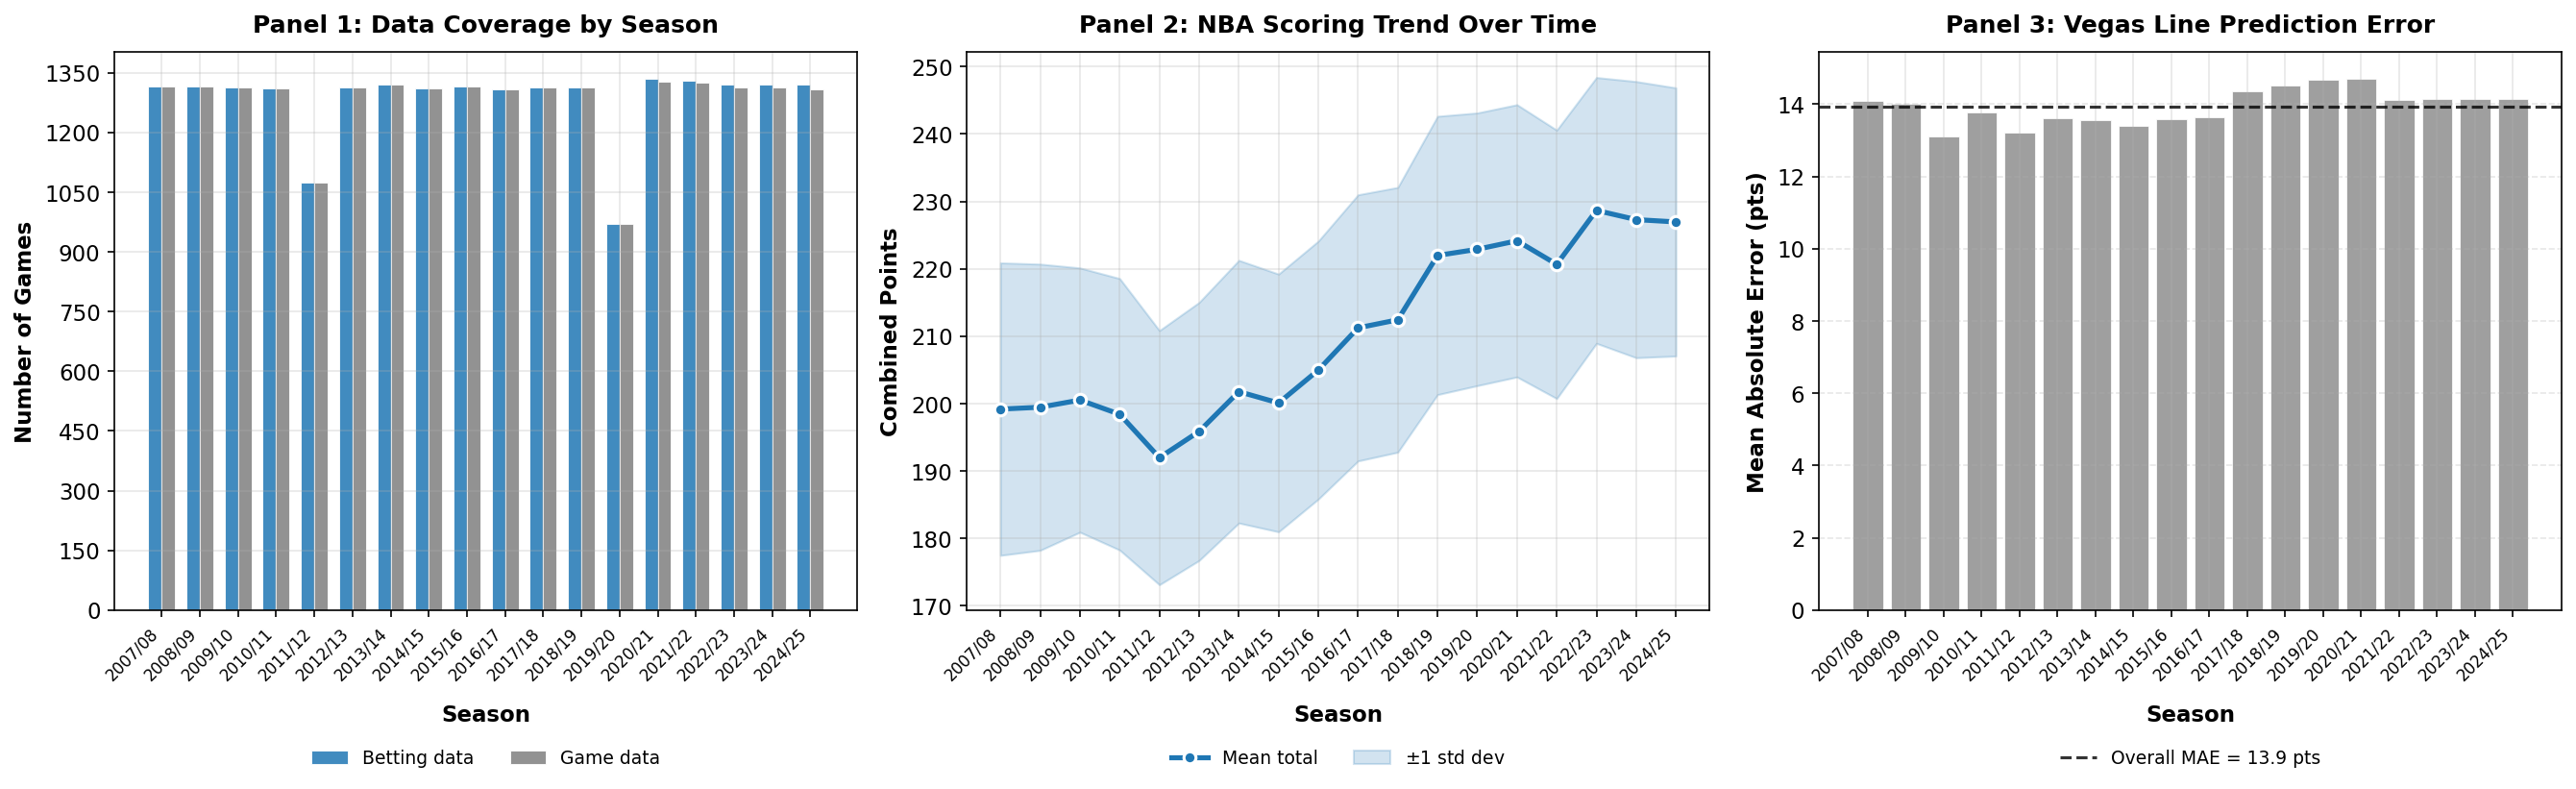
\includegraphics[width=0.90\linewidth]{Images/notitle/nofig01_data_overview.png}
    \caption{Data coverage by season (Panel 1), secular rise in NBA scoring (Panel 2), and Vegas line MAE across seasons (Panel 3).}
    \label{fig:1}
\end{figure}

Figure~\ref{fig:1} confirms consistent coverage of ${\sim}$1,200--1,300 games per season. The Vegas line's MAE has remained stable at 14--17 points, implying that any model edge is unlikely to stem from simple scoring-level shifts.

\subsection{Why Machine Learning Might Find an Edge}
In an efficient market, the Vegas line should already incorporate all public information. However, three structural features suggest a potential opening. First, team-level rolling statistics (form over 5 and 10 games) may contain lagged information the market prices slowly---analogous to \emph{momentum} in equity markets, where recent performance tends to persist. If the Vegas line reacts to form shifts with even a one- or two-game delay, a model conditioning on the most recent data has an opportunity. Second, interaction features (e.g., pace $\times$ pace, rest asymmetry $\times$ home-court) capture non-additive matchup effects that an oddsmaker setting 15 lines per night may underweight---analogous to \emph{factor investing}, where systematic strategies exploit dimensions of return that individual analysts overlook. Third, the residual error ($\text{MAE} \approx 15$ points) is large relative to the line itself (${\sim}220$ points), leaving room for any model that can explain even a small fraction of this residual.

%% =====================================================================
%%  SECTION 3: FEATURE ENGINEERING
%% =====================================================================
\section{Feature Engineering}
Feature engineering transforms raw game data into 114 numerical inputs in seven categories: Vegas line features (3), totals/scoring (18), shooting efficiency (24), rebounding/hustle (16), playmaking (8), schedule/rest (11), context indicators (6), and interaction features (28). All features are strictly lagged via a \texttt{shift(1)} operation within each season, preventing lookahead bias. Rolling averages use two windows: L5 (last 5 games) for short-term form and L10 for medium-term stability. Pace is estimated as $\text{FGA} - \text{OREB} + \text{TOV} + 0.44 \times \text{FTA}$. Interaction features allow linear models to capture non-additive effects. All features are z-scored using training-set statistics only, preventing test-set information leakage.

\begin{figure}[H]
    \centering
    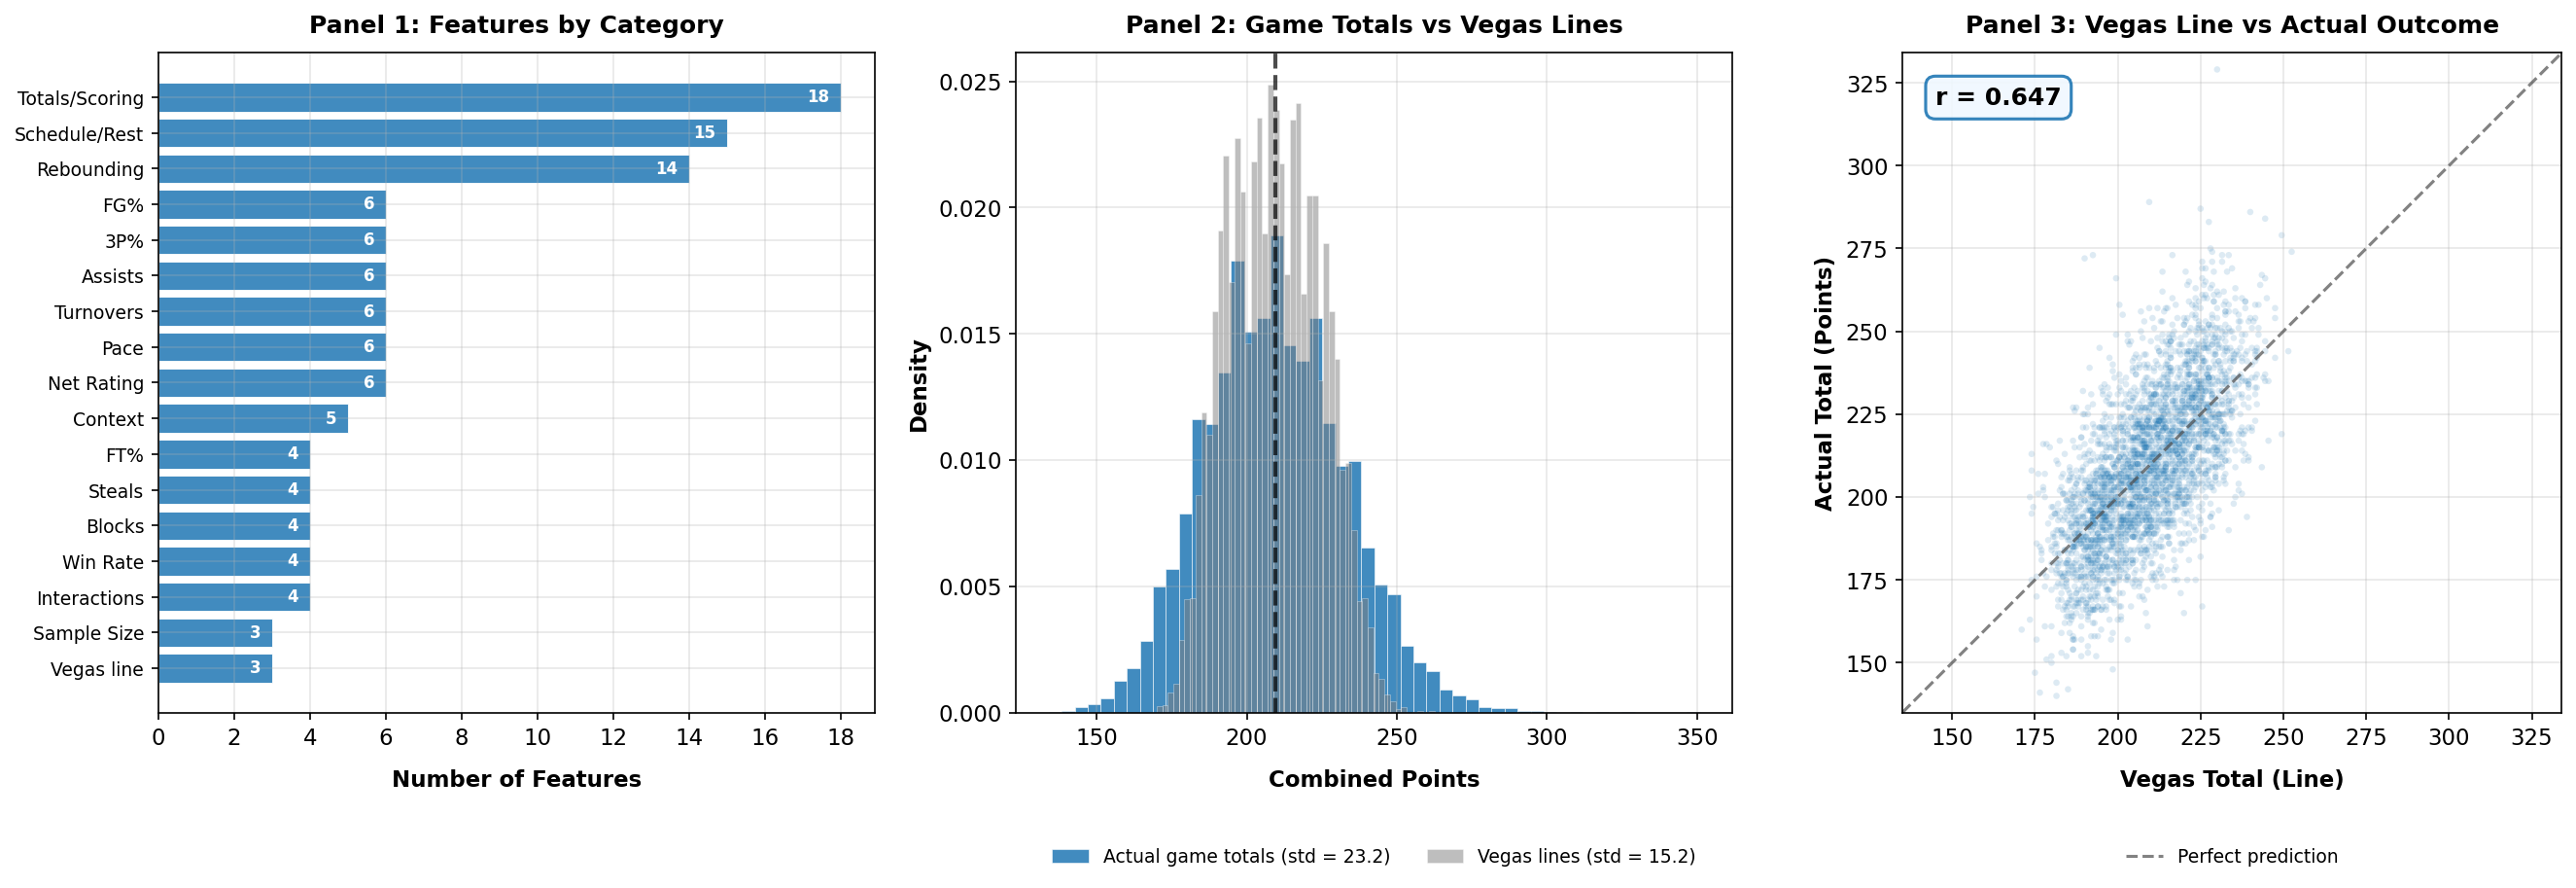
\includegraphics[width=0.90\linewidth]{Images/notitle/nofig02_feature_matrix_overview.png}
    \caption{Feature composition by category (Panel 1), distribution of game totals vs.\ the Vegas line (Panel 2), and Vegas line predictions vs.\ actual outcomes (Panel 3).}
    \label{fig:2}
\end{figure}

Figure~\ref{fig:2} confirms the feature set is dominated by scoring and shooting metrics, and that the Vegas line is a strong but imperfect predictor ($r \approx 0.65$).

%% =====================================================================
%%  SECTION 4: MODEL TRAINING AND WALK-FORWARD EVALUATION
%% =====================================================================
\section{Model Training and Walk-Forward Evaluation}
Walk-forward backtesting enforces strict temporal ordering: for each of 11 test seasons (2013/14--2023/24), the model trains on all prior data and predicts the test season. The training set grows by ${\sim}$1,300 games per iteration. Hyperparameters are tuned via 5-fold \texttt{TimeSeriesSplit}, optimising betting accuracy rather than RMSE---because minimising regression error does not necessarily maximise the binary over/under decision that drives profit.

\vspace{2pt}
\begin{table}[H]
\centering\small
\begin{tabularx}{\linewidth}{llX}
\toprule
\textbf{Model} & \textbf{Family} & \textbf{Core Idea} \\
\midrule
Ridge & Linear + L2 & Shrinks all coefficients toward zero; handles correlated features gracefully. \\
Lasso & Linear + L1 & Drives some coefficients exactly to zero---automatic feature selection. \\
ElasticNet & L1 + L2 & Combines Lasso's sparsity with Ridge's stability for correlated features. \\
PCR & PCA + Ridge & Reduces dimensionality first, then applies Ridge in lower-dimensional space. \\
XGBoost & Boosted trees & Learns nonlinear patterns via sequential decision trees. \\
RBF+Ridge & Kernel + Ridge & Maps features into high-dimensional space where nonlinear patterns become linear. \\
\bottomrule
\end{tabularx}
\end{table}
\vspace{-2pt}

Several design choices are noteworthy. First, \emph{exponential recency weighting} controlled by a half-life parameter allows models to adapt to the NBA's evolving scoring environment; older games receive less weight, with the decay rate tuned jointly with model hyperparameters. For Ridge, Lasso, and ElasticNet, a full joint grid over half-life and regularisation strength is searched. For PCR, the one-standard-error (1SE) rule selects the simplest model within one standard deviation of the best CV score, favouring parsimony against overfitting. For XGBoost and RBF+Ridge, a sequential two-stage procedure first tunes the half-life, then tunes model-specific parameters. Second, all features are standardised (z-scored) using training-set statistics only---the test data is transformed using these same statistics, preventing any leakage. Pooling predictions across all 11 seasons yields ${\sim}$14,000 out-of-sample bets per model.

\begin{figure}[H]
    \centering
    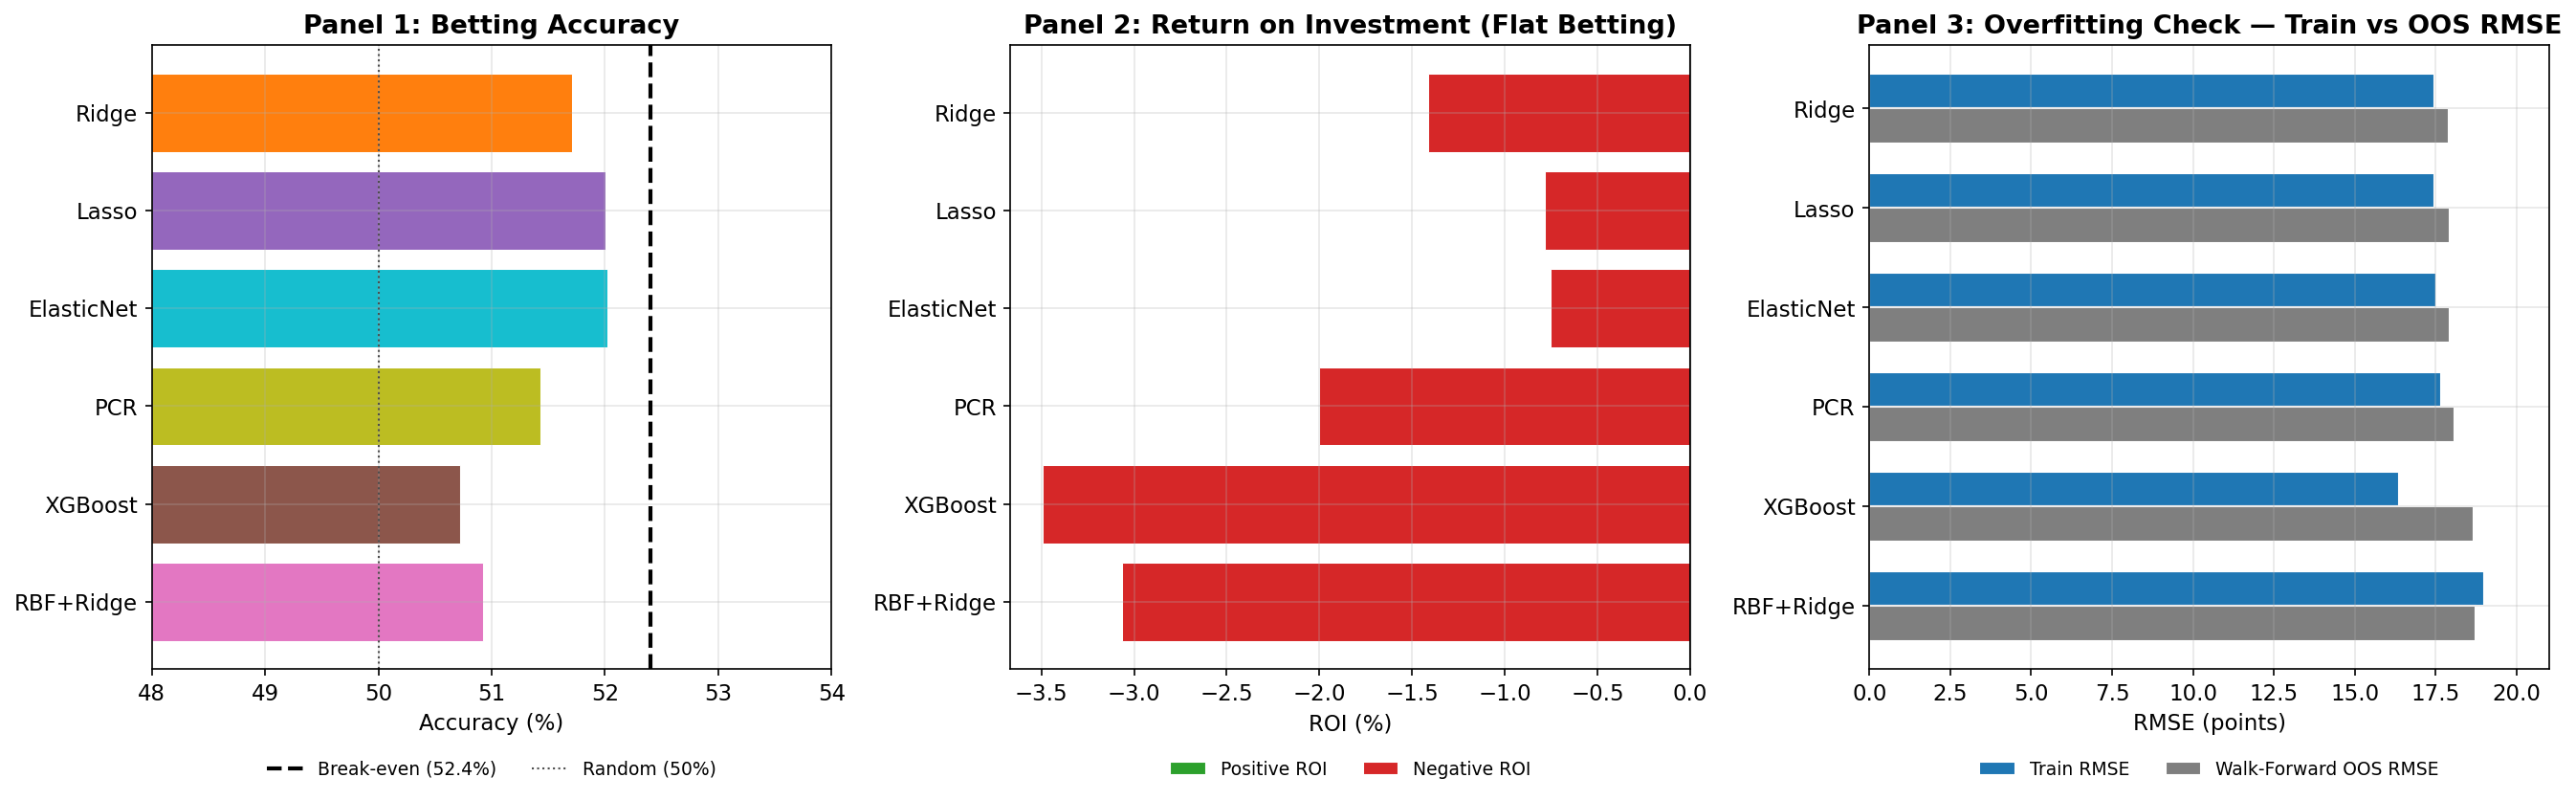
\includegraphics[width=0.90\linewidth]{Images/notitle/nofig03_model_comparison.png}
    \caption{Walk-forward results: betting accuracy (Panel 1), ROI at $-110$ odds (Panel 2), and overfitting diagnostics via train vs.\ OOS RMSE (Panel 3).}
    \label{fig:3}
\end{figure}

\subsection{Key Findings}
All six models cluster between $50.7\%$ and $52.0\%$ accuracy. The linear models (Ridge $51.7\%$, Lasso and ElasticNet $52.0\%$) lead; XGBoost ($50.7\%$) and RBF+Ridge ($50.9\%$) trail. No model reaches the $52.4\%$ break-even threshold when betting every game. The overfitting check (Figure~\ref{fig:3}, Panel~3) shows linear models have minimal train-vs-OOS RMSE gaps (${\sim}0.4$ points), while XGBoost shows a 2.3-point gap---confirming it memorises training patterns that do not generalise. This is the \emph{bias-variance tradeoff} in action: in a low-signal environment, model flexibility becomes a liability. In financial terms, many quantitative strategies show significant alpha before transaction costs but lose money after commissions and slippage; our results exhibit the same pattern.

\begin{figure}[H]
    \centering
    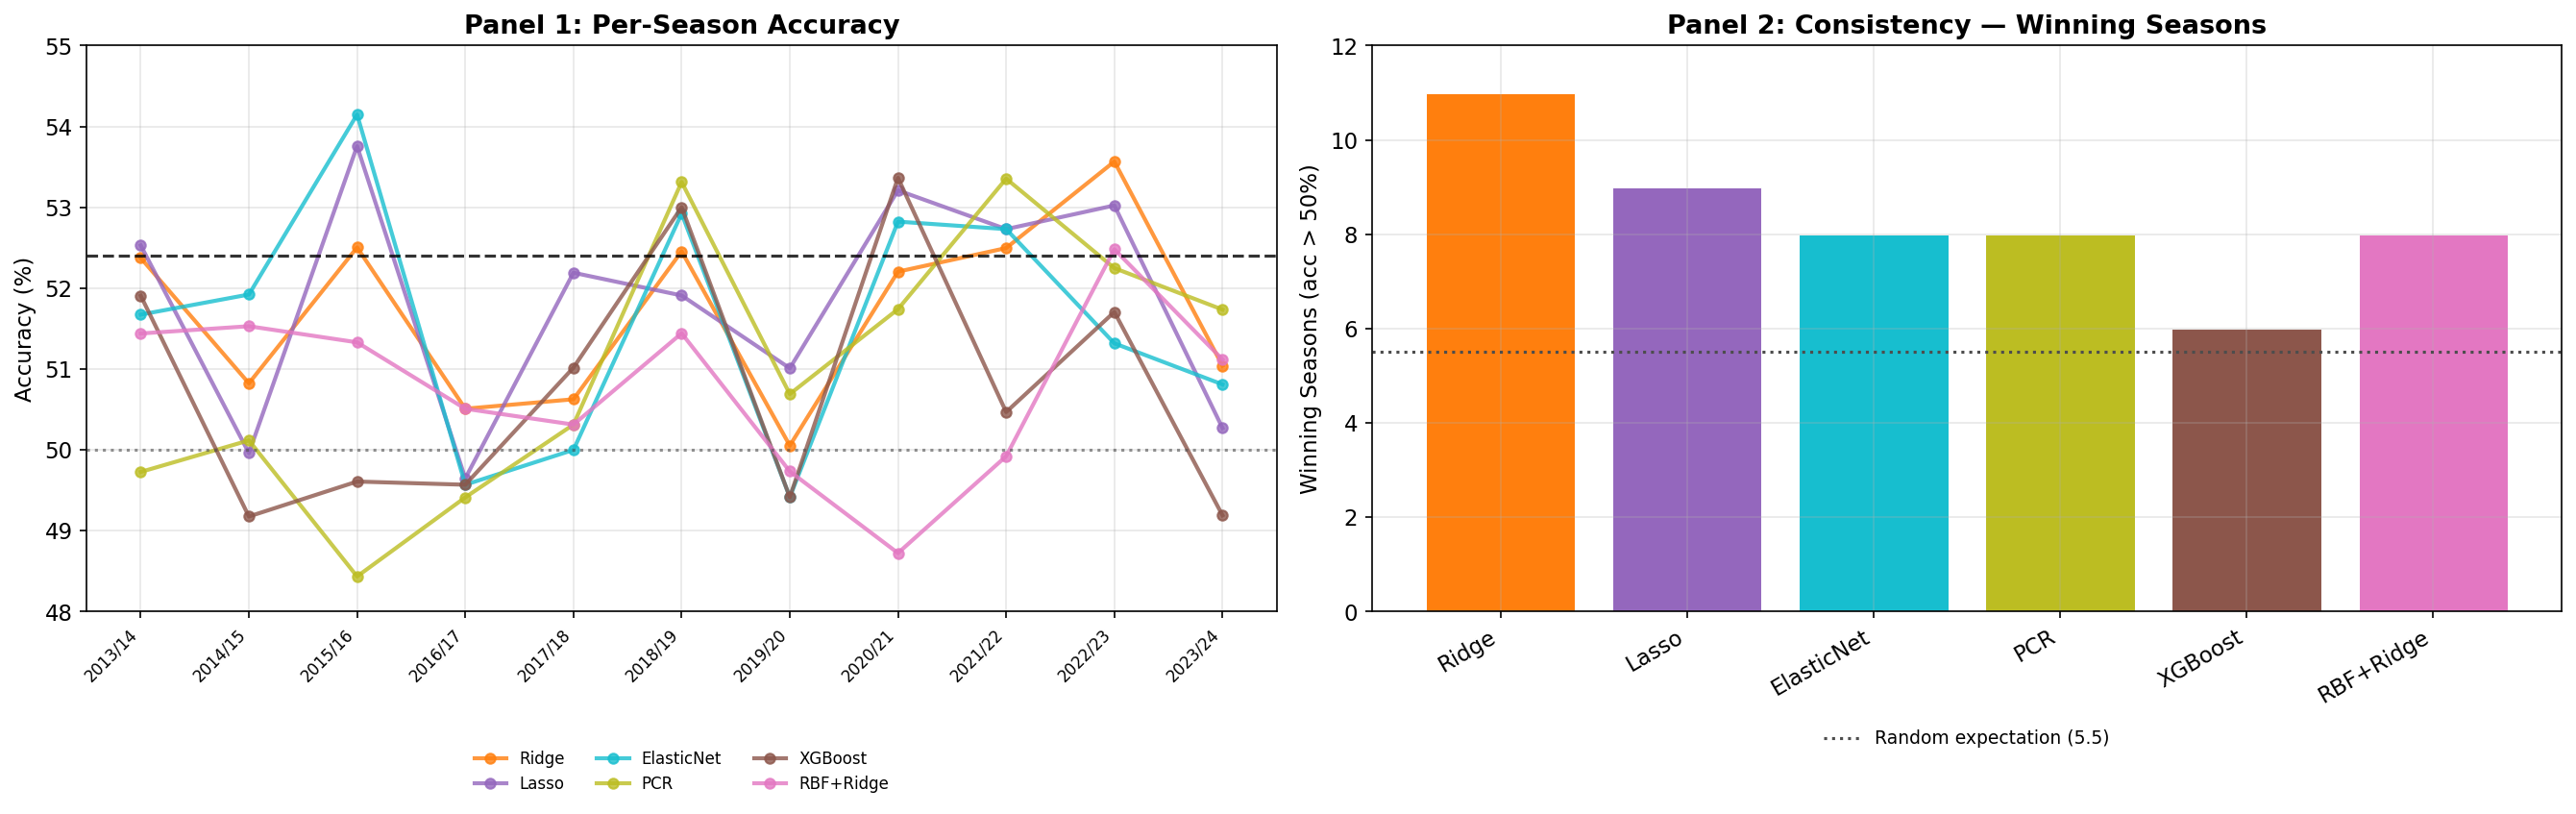
\includegraphics[width=0.90\linewidth]{Images/notitle/nofig04_per_season_accuracy.png}
    \caption{Per-season accuracy (Panel 1) and winning-season consistency (Panel 2) across 11 walk-forward test seasons.}
    \label{fig:4}
\end{figure}

Per-season analysis (Figure~\ref{fig:4}) reveals volatile accuracy (48--55\%), with no model consistently beating $52.4\%$ across all seasons. Lasso achieves the highest above-$50\%$ season count (10 of 11).

%% =====================================================================
%%  SECTION 5: STATISTICAL SIGNIFICANCE TESTING
%% =====================================================================
\section{Statistical Significance Testing}
With over 14,000 bets per model, even small deviations from $50\%$ require formal testing. We apply \emph{Wilson score confidence intervals}, \emph{block bootstrap} resampling (preserving temporal correlation via contiguous 50-game blocks), and \emph{Bonferroni correction} for testing six models simultaneously ($p < 0.05/6 \approx 0.0083$).

\begin{figure}[H]
    \centering
    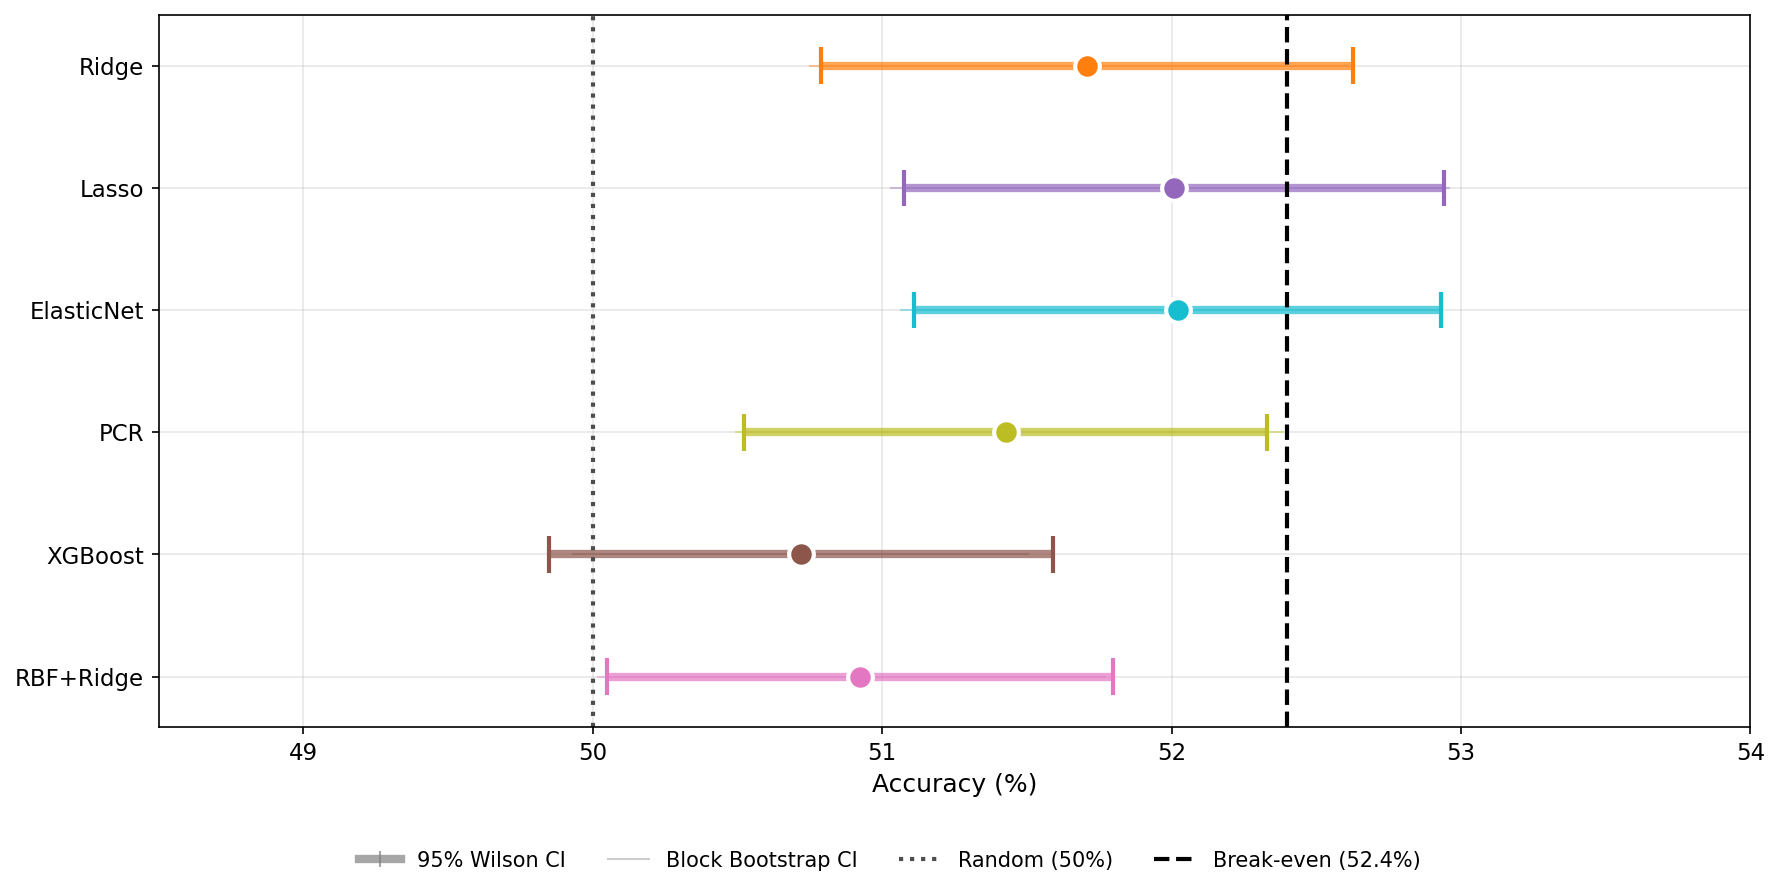
\includegraphics[width=0.55\linewidth]{Images/notitle/nofig05_statistical_validation.png}
    \caption{95\% CIs for model accuracy. Dashed lines mark $50\%$ (chance) and $52.4\%$ (break-even).}
    \label{fig:5}
\end{figure}

After Bonferroni correction, four models are significantly above $50\%$: Ridge, Lasso, ElasticNet, and PCR (all $p < 0.006$). RBF+Ridge loses significance after correction (adjusted $p \approx 0.12$); XGBoost fails even before correction ($p \approx 0.054$). All three CI methods produce nearly identical intervals, confirming temporal correlation does not inflate confidence. Critically, every model's CI includes $52.4\%$---we cannot confirm profitability with flat betting at $95\%$ confidence.

%% =====================================================================
%%  SECTION 6: SELECTIVE BETTING WITH CONFIDENCE THRESHOLDS
%% =====================================================================
\section{Selective Betting with Confidence Thresholds}
Since no model is profitable betting every game, we test whether restricting bets to games where the model strongly disagrees with Vegas can push accuracy above break-even. The confidence measure is $|\hat{y} - \text{Vegas}|$, swept from $0.5$ to 20 points, subject to dual validity constraints: $\geq 300$ total bets and $\geq 10$ bets in every season. ROI at $-110$ odds is:
\vspace{-4pt}
$$\text{ROI} = \frac{\text{Wins} \times \$100 \;-\; \text{Losses} \times \$110}{\text{Number of Bets} \times \$100}$$
\vspace{-6pt}

\noindent Break-even ROI $= 0\%$ corresponds to $52.4\%$ accuracy.

\begin{figure}[H]
    \centering
    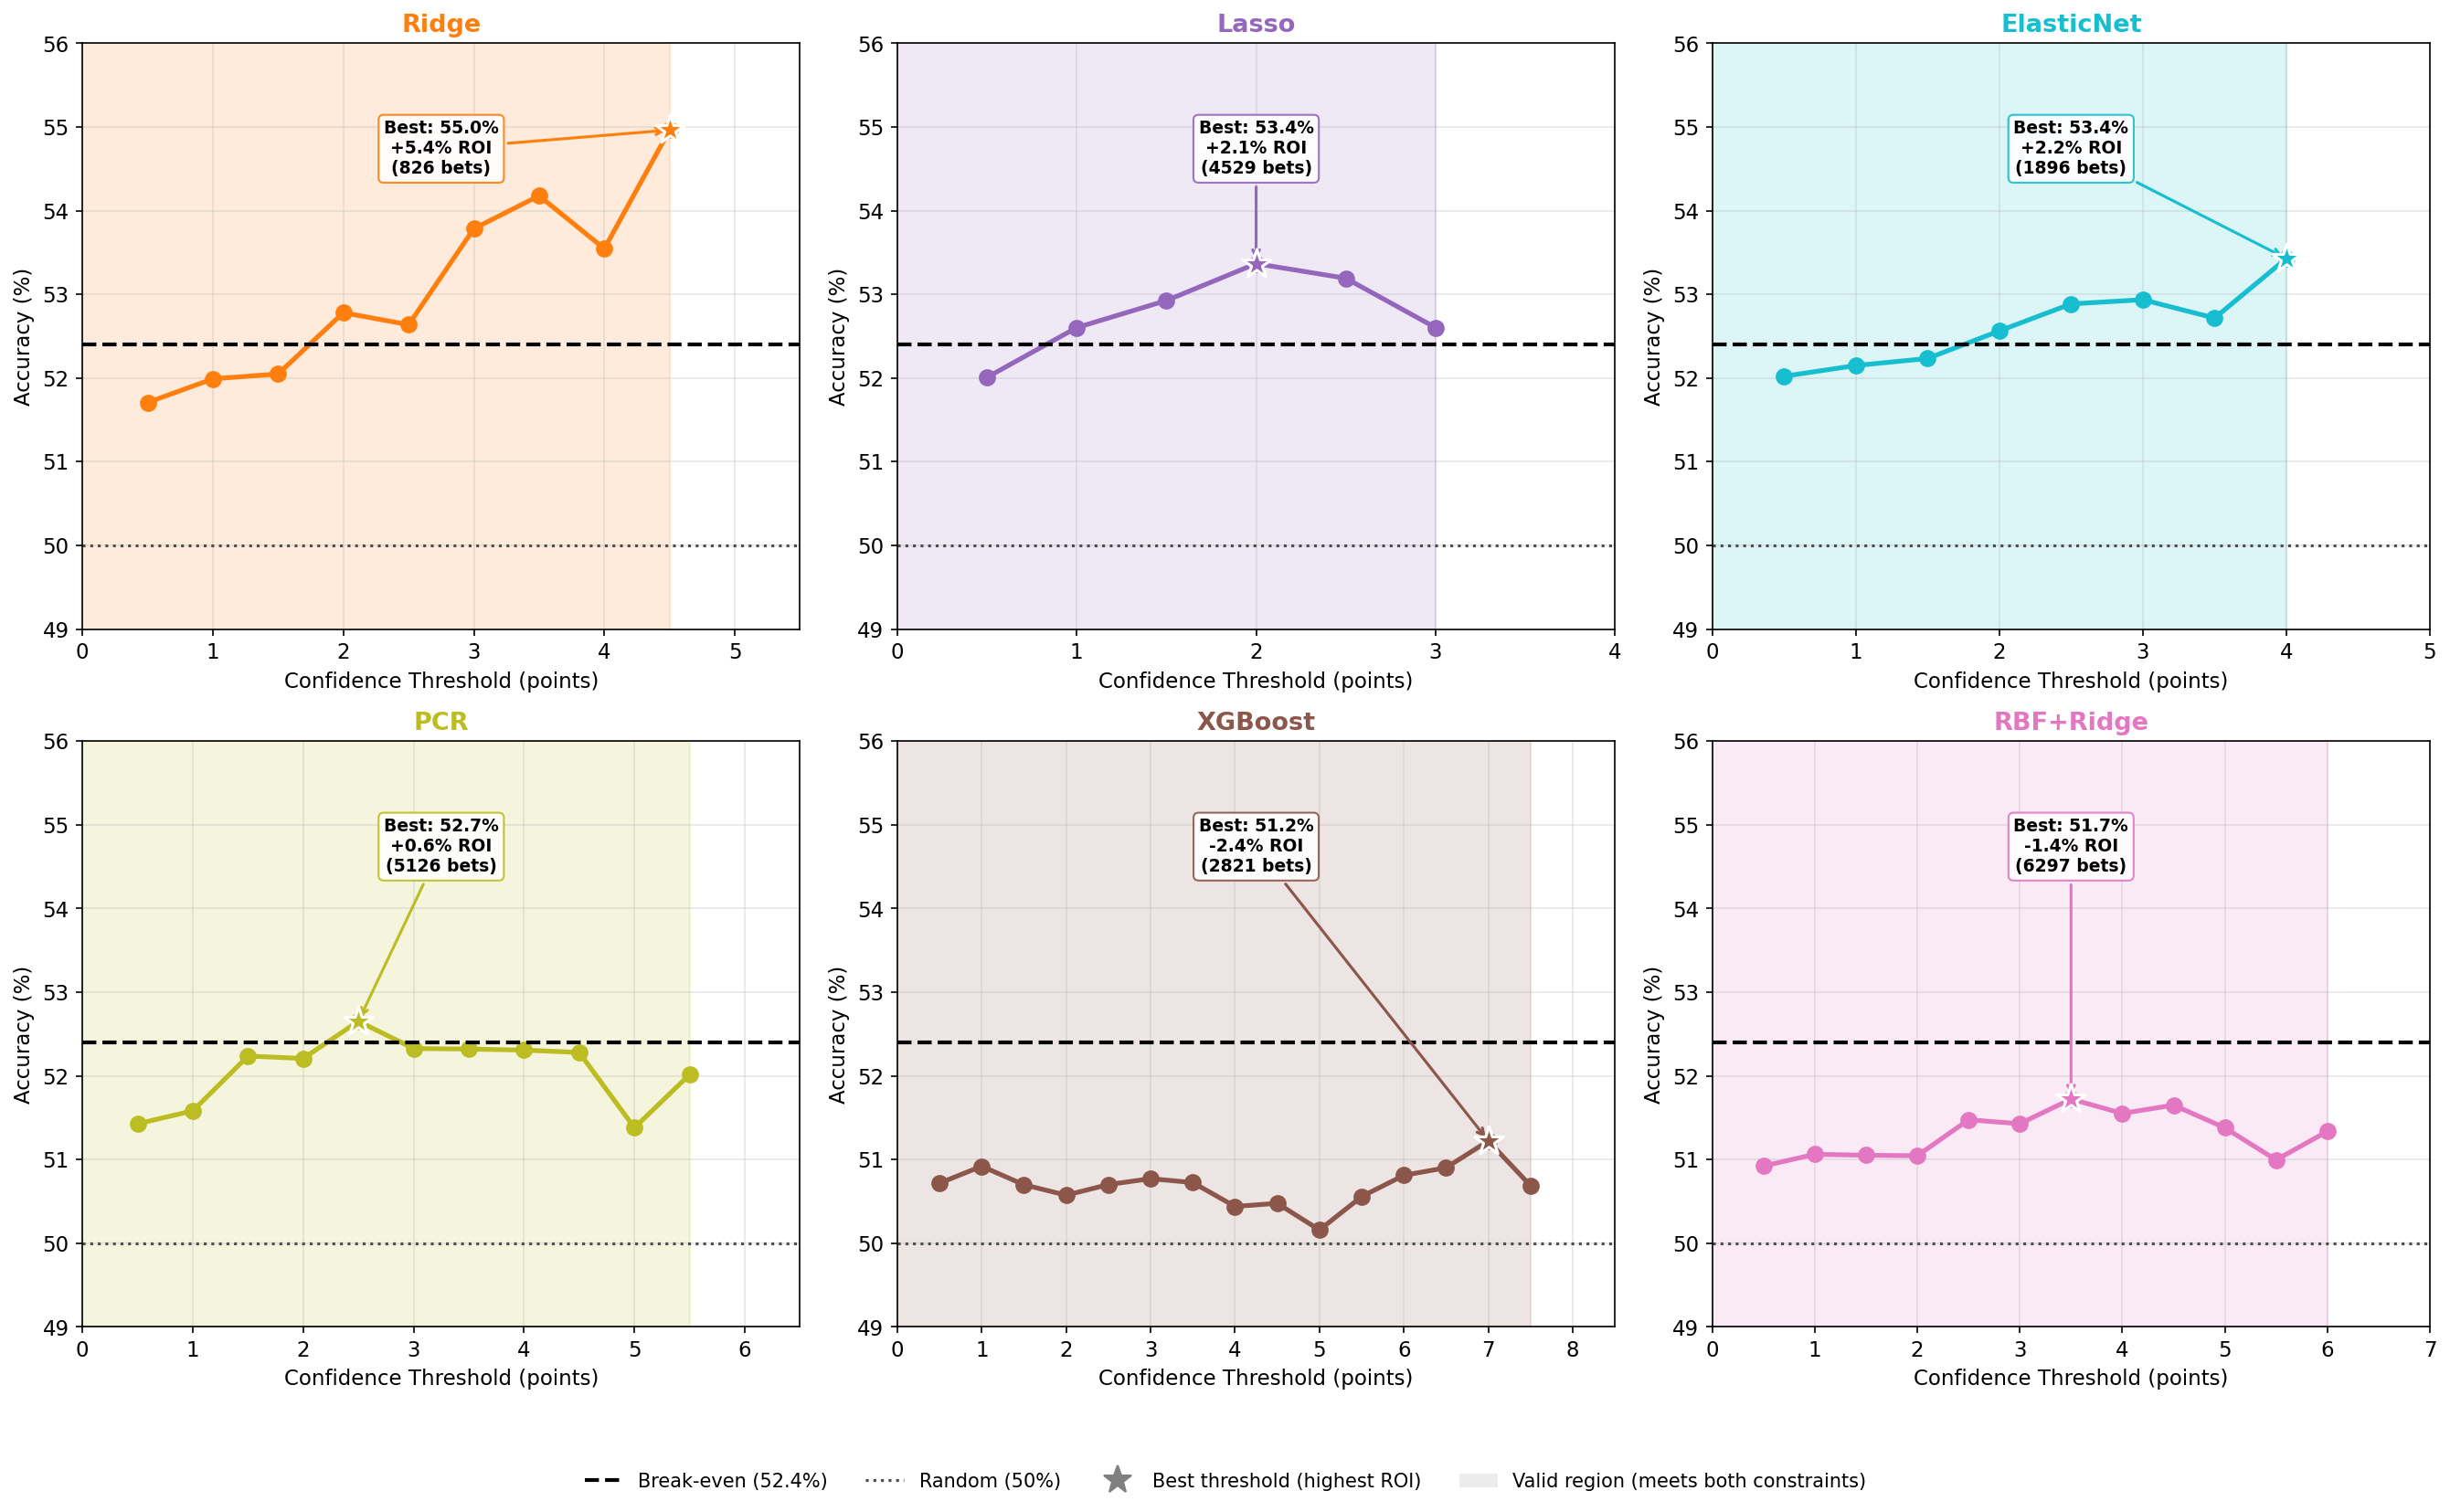
\includegraphics[width=0.90\linewidth]{Images/notitle/nofig06_threshold_accuracy_grid.png}
    \caption{Per-model accuracy by confidence threshold. Green shading = valid regions; stars = optimal thresholds.}
    \label{fig:6}
\end{figure}
\vspace{-4pt}
\begin{figure}[H]
    \centering
    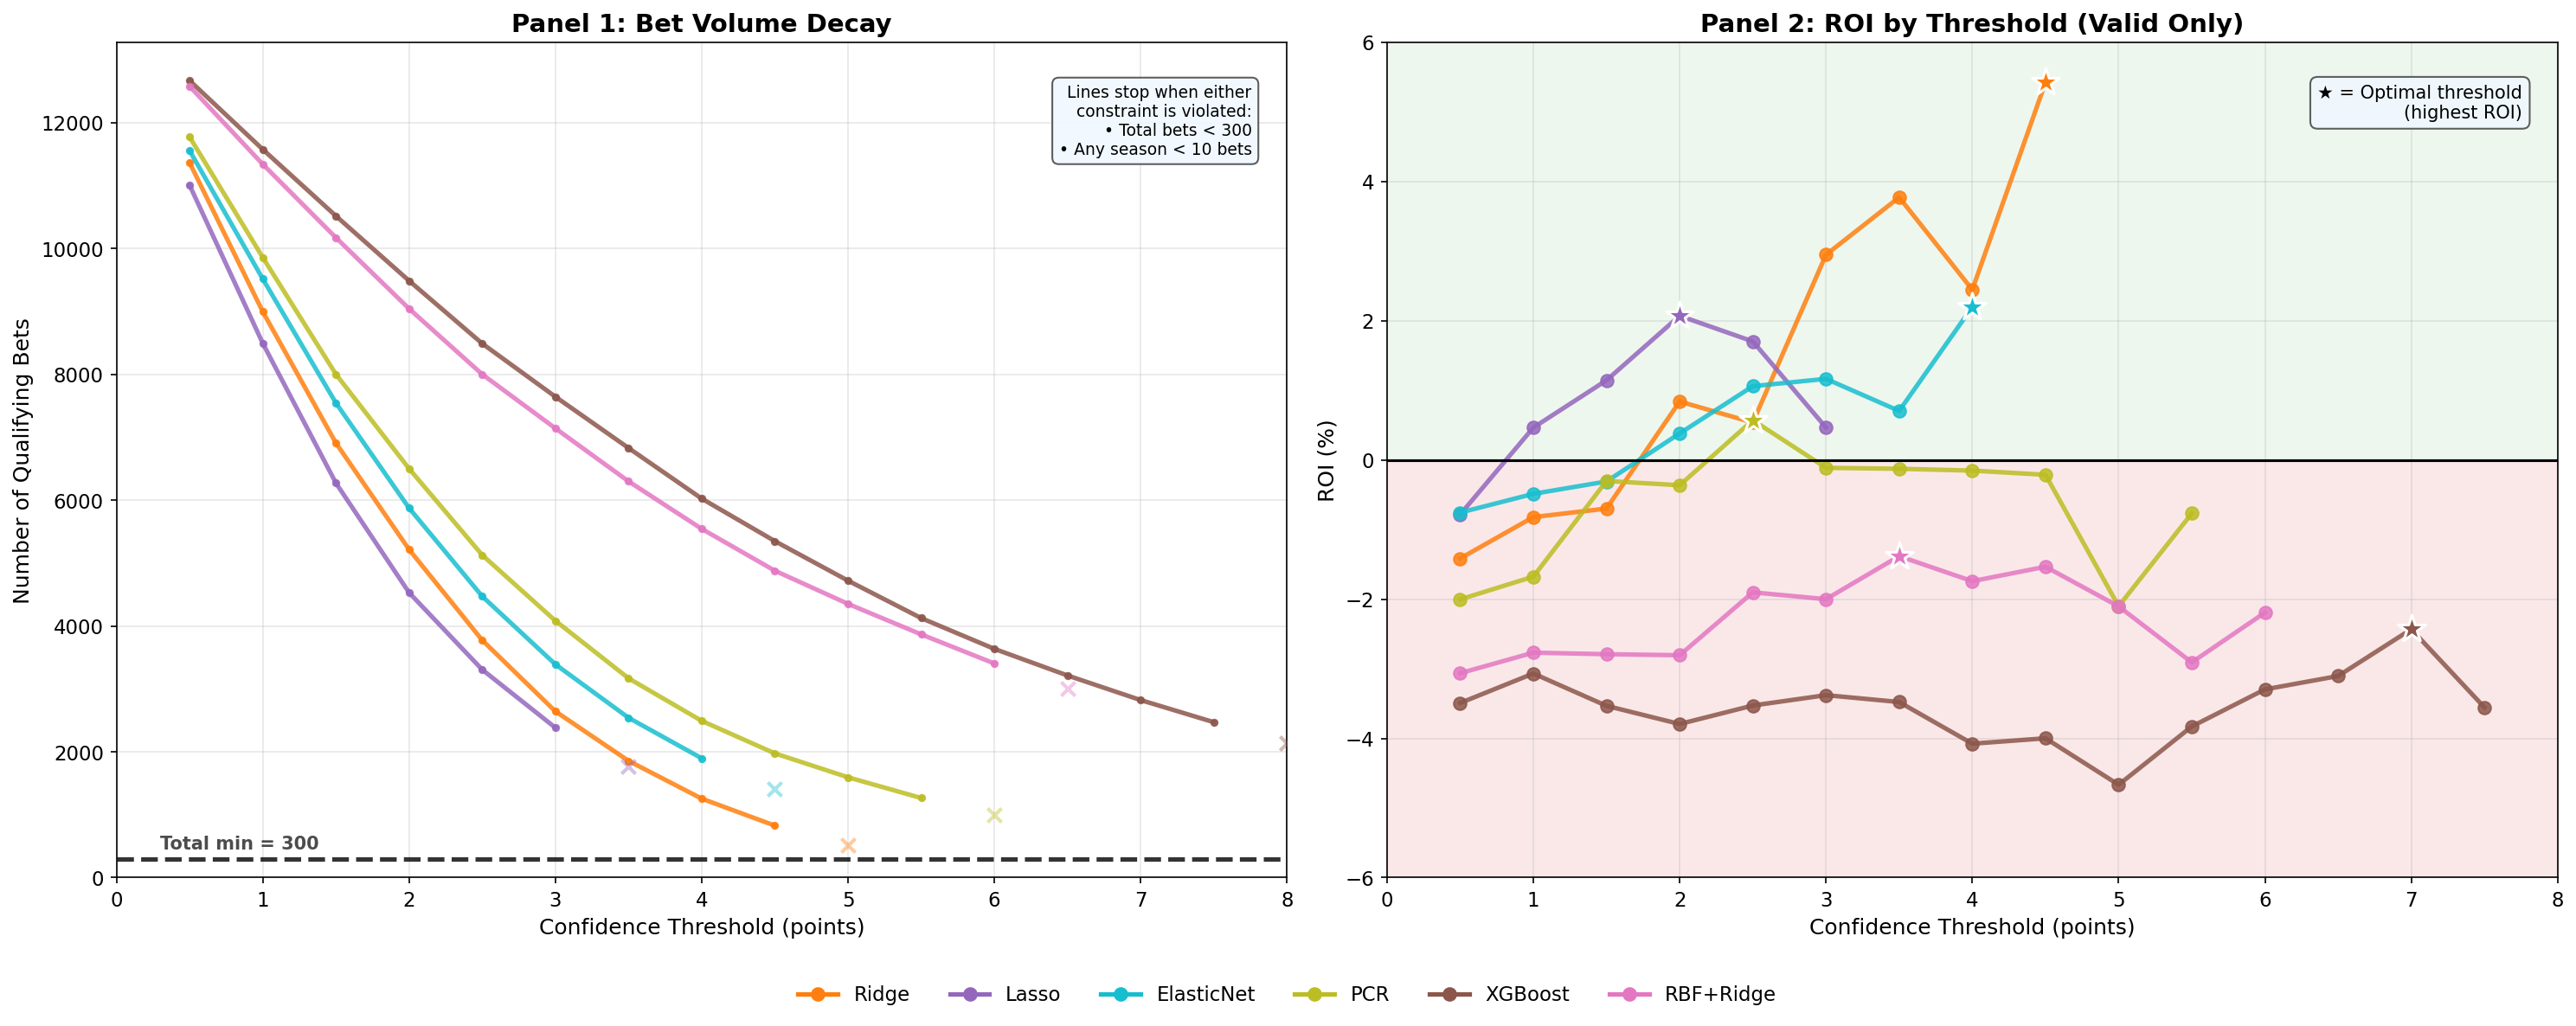
\includegraphics[width=0.90\linewidth]{Images/notitle/nofig07_threshold_overview.png}
    \caption{Bet volume decay (Panel 1) and ROI by threshold (Panel 2).}
    \label{fig:7}
\end{figure}

Four models achieve positive ROI: Ridge at $+5.4\%$ ($55.0\%$ accuracy, 826 bets, threshold $\geq 4.5$), ElasticNet $+2.2\%$ (1,896 bets, $\geq 4.0$), Lasso $+2.1\%$ (4,529 bets, $\geq 2.0$), and PCR $+0.6\%$ (5,126 bets, $\geq 2.5$). XGBoost and RBF+Ridge never achieve positive ROI.

\subsection{Prediction Variance Explains Model Differences}
Linear models produce predictions with standard deviations of 2.4--2.8 points, making conservative adjustments to the Vegas line---when they strongly disagree, it likely reflects genuine signal. XGBoost and RBF+Ridge have standard deviations of ${\sim}5.8$--$5.9$ points (${\sim}2.5\times$ larger), routinely producing extreme predictions driven by overfitting. Selectivity cannot separate signal from noise when predictions themselves are noisy.

\begin{figure}[H]
    \centering
    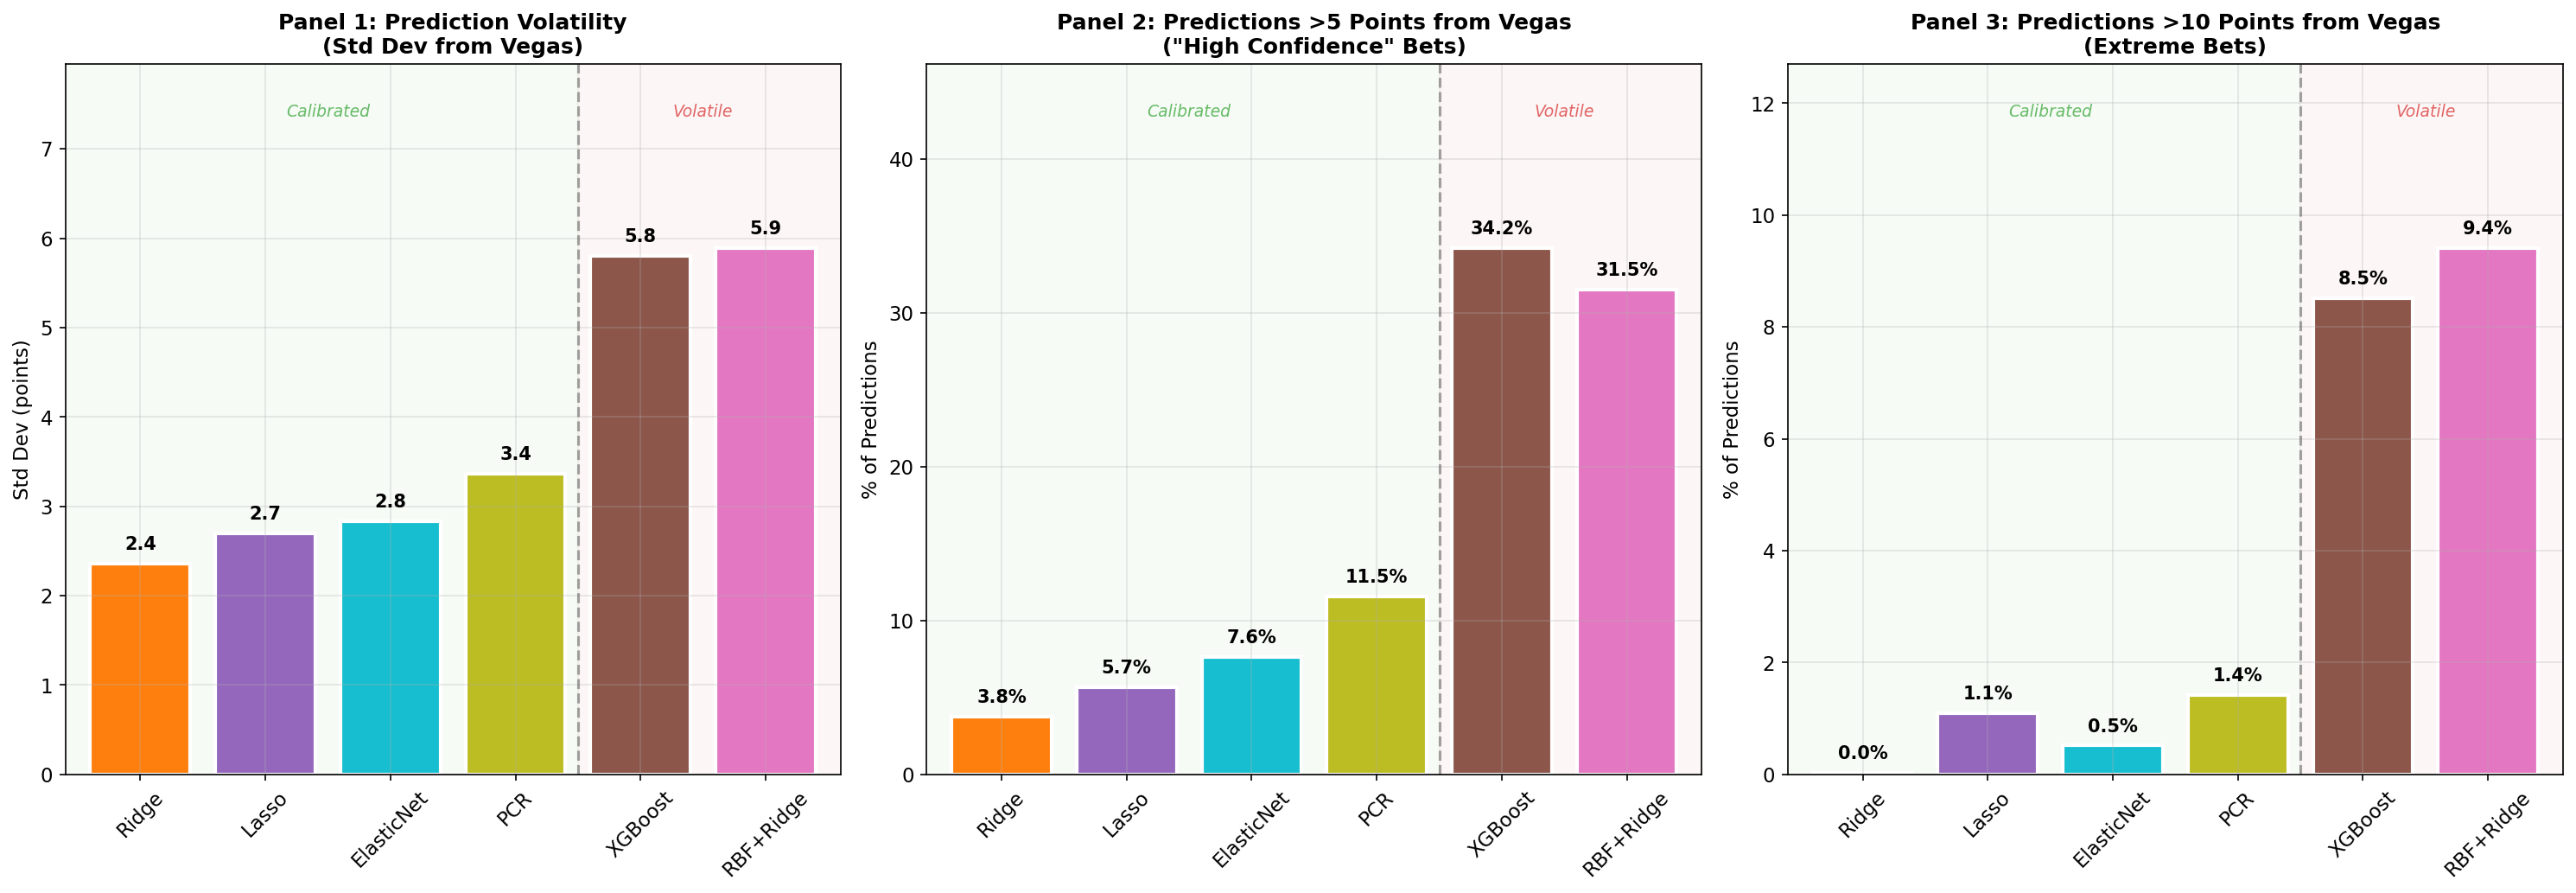
\includegraphics[width=0.90\linewidth]{Images/notitle/nofig08_prediction_variance.png}
    \caption{Prediction variance: standard deviation, fraction $>5$ points from Vegas, and fraction $>10$ points.}
    \label{fig:8}
\end{figure}
\vspace{-4pt}
\begin{figure}[H]
    \centering
    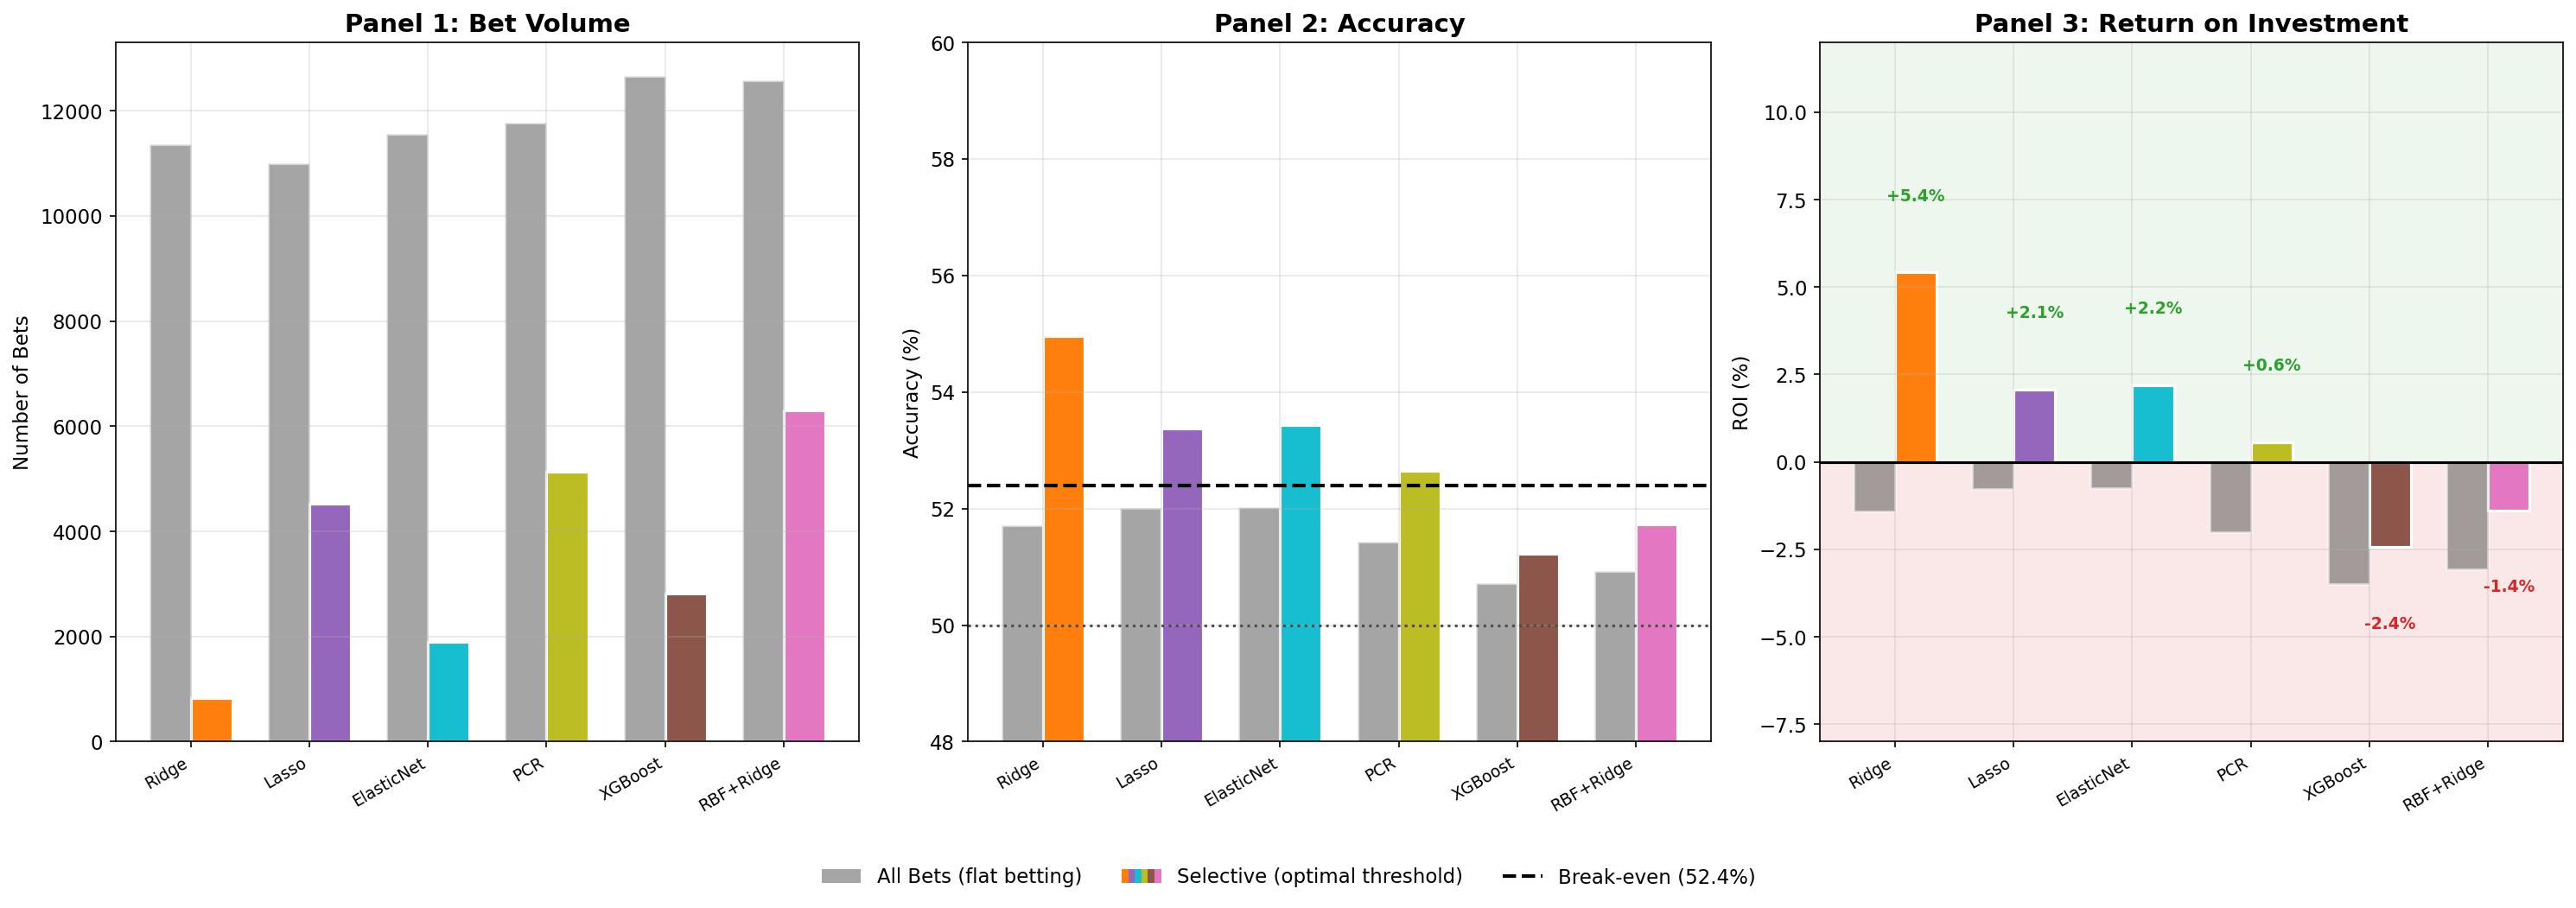
\includegraphics[width=0.90\linewidth]{Images/notitle/nofig09_base_vs_selective.png}
    \caption{Base vs.\ selective betting: volume reduction (Panel 1), accuracy improvement (Panel 2), ROI shift (Panel 3).}
    \label{fig:9}
\end{figure}

Four models flip from negative to positive ROI with selectivity (Figure~\ref{fig:9}). However, selective betting widens confidence intervals due to reduced sample sizes. After Bonferroni correction, no model's selective accuracy is significantly above $52.4\%$---the evidence is suggestive but not conclusive.

\begin{figure}[H]
    \centering
    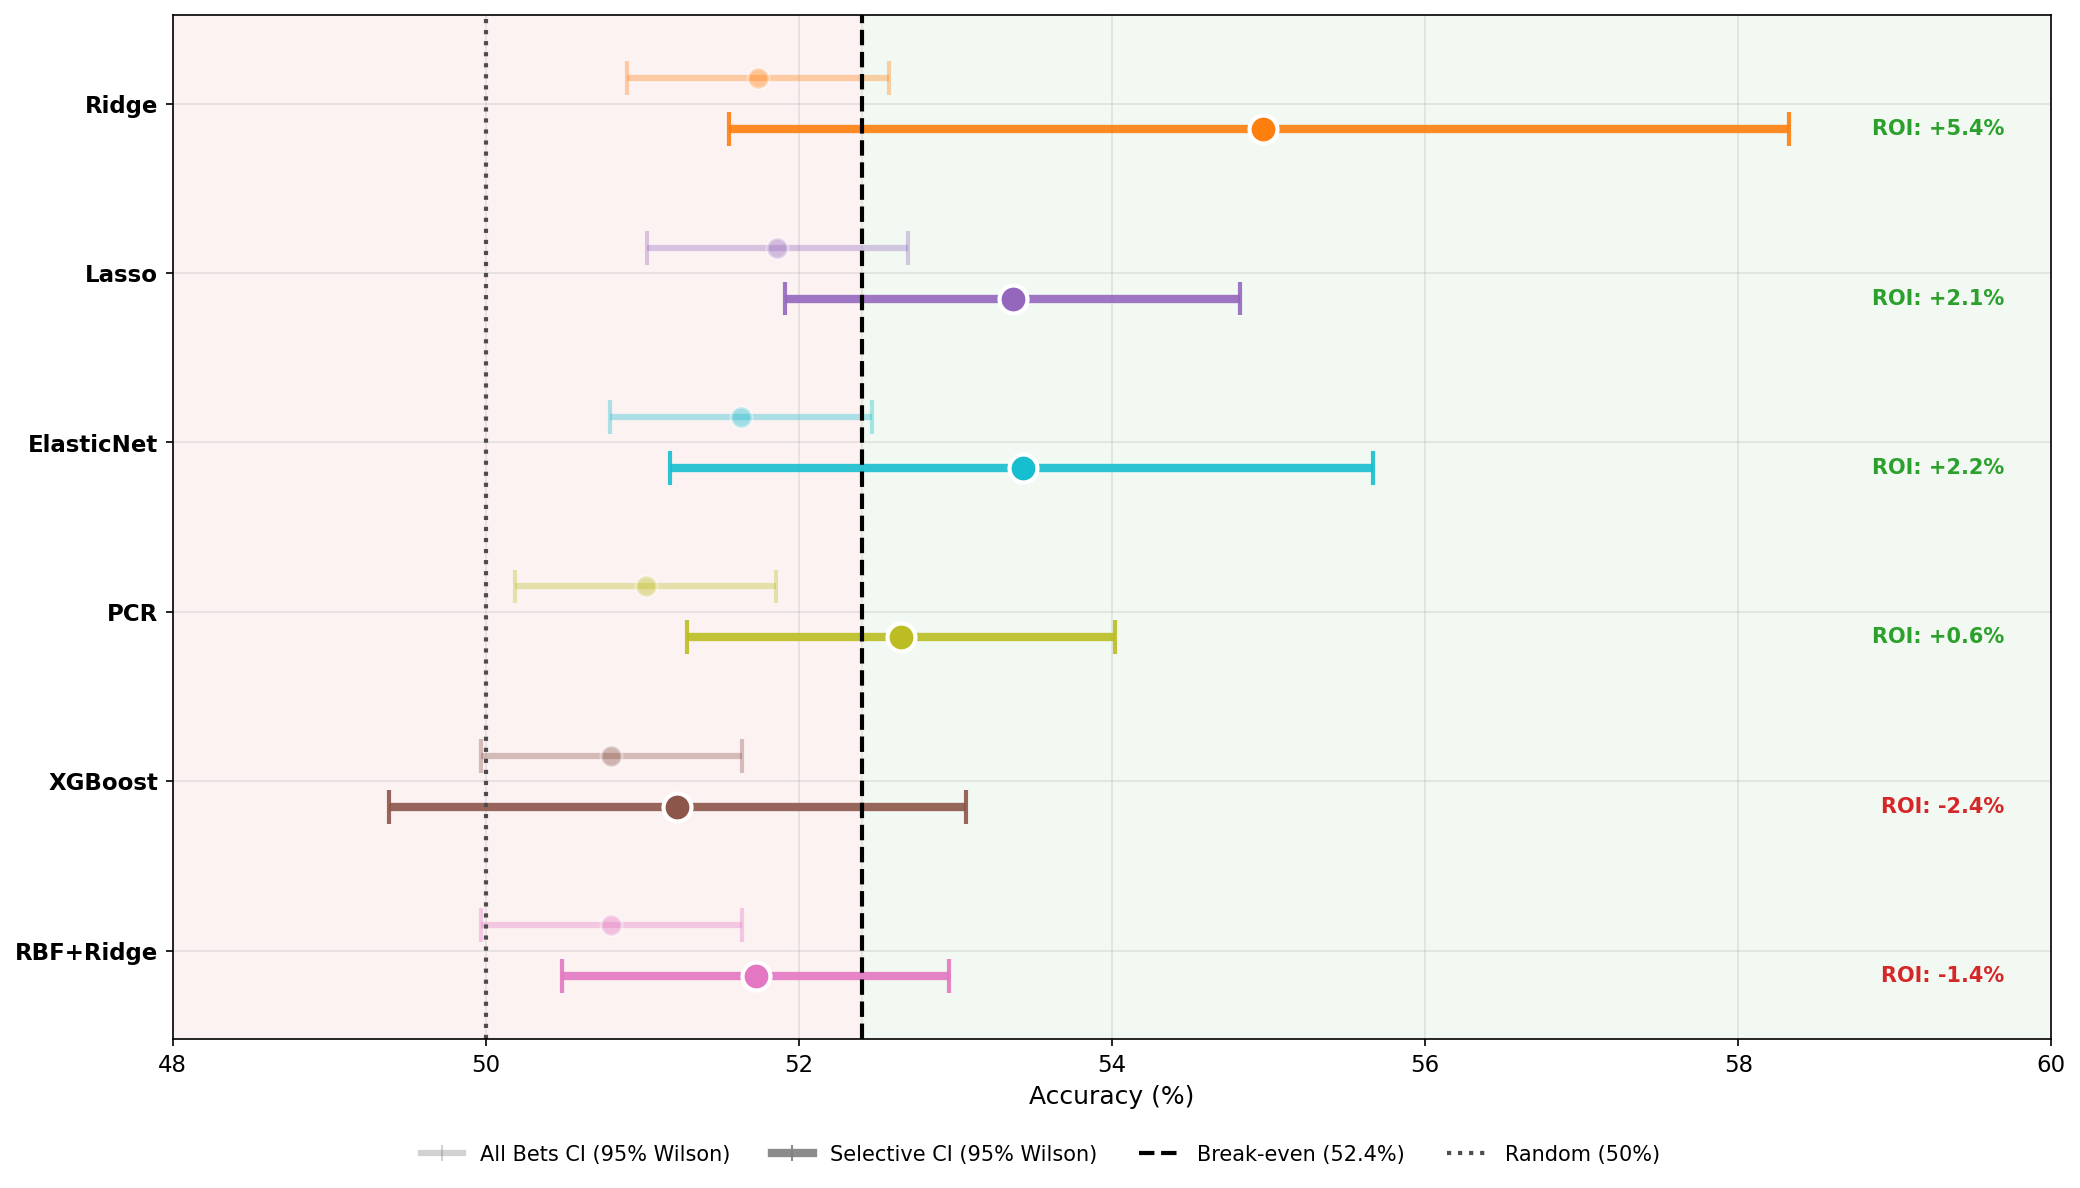
\includegraphics[width=0.55\linewidth]{Images/notitle/nofig10_selective_ci_comparison.png}
    \caption{CIs for base vs.\ selective accuracy. Selectivity improves point estimates but widens intervals.}
    \label{fig:10}
\end{figure}

%% =====================================================================
%%  SECTION 7: BANKROLL SIMULATION AND BET SIZING
%% =====================================================================
\section{Bankroll Simulation and Bet Sizing}
The four qualifying models are subjected to bankroll simulations across 10 sizing rules in three families: flat dollar amounts (1\%, 2\%, 5\% of initial bankroll), proportional sizing (1\%, 2\%, 5\% of current bankroll), and the Kelly criterion with full, half, and quarter fractions plus a 5\%-capped variant. Starting bankroll: \$10,000.

The Kelly criterion maximises long-run compound growth: $f^{*} = (bp - q)/b$, where $b = 100/110 \approx 0.909$, $p$ = win probability, $q = 1-p$. For Ridge at $p = 0.550$: $f^* = 5.50\%$. However, Kelly is optimal only when $p$ is known exactly; with standard errors of 1--3pp, fractional Kelly (half, quarter) is preferred.

\begin{figure}[H]
    \centering
    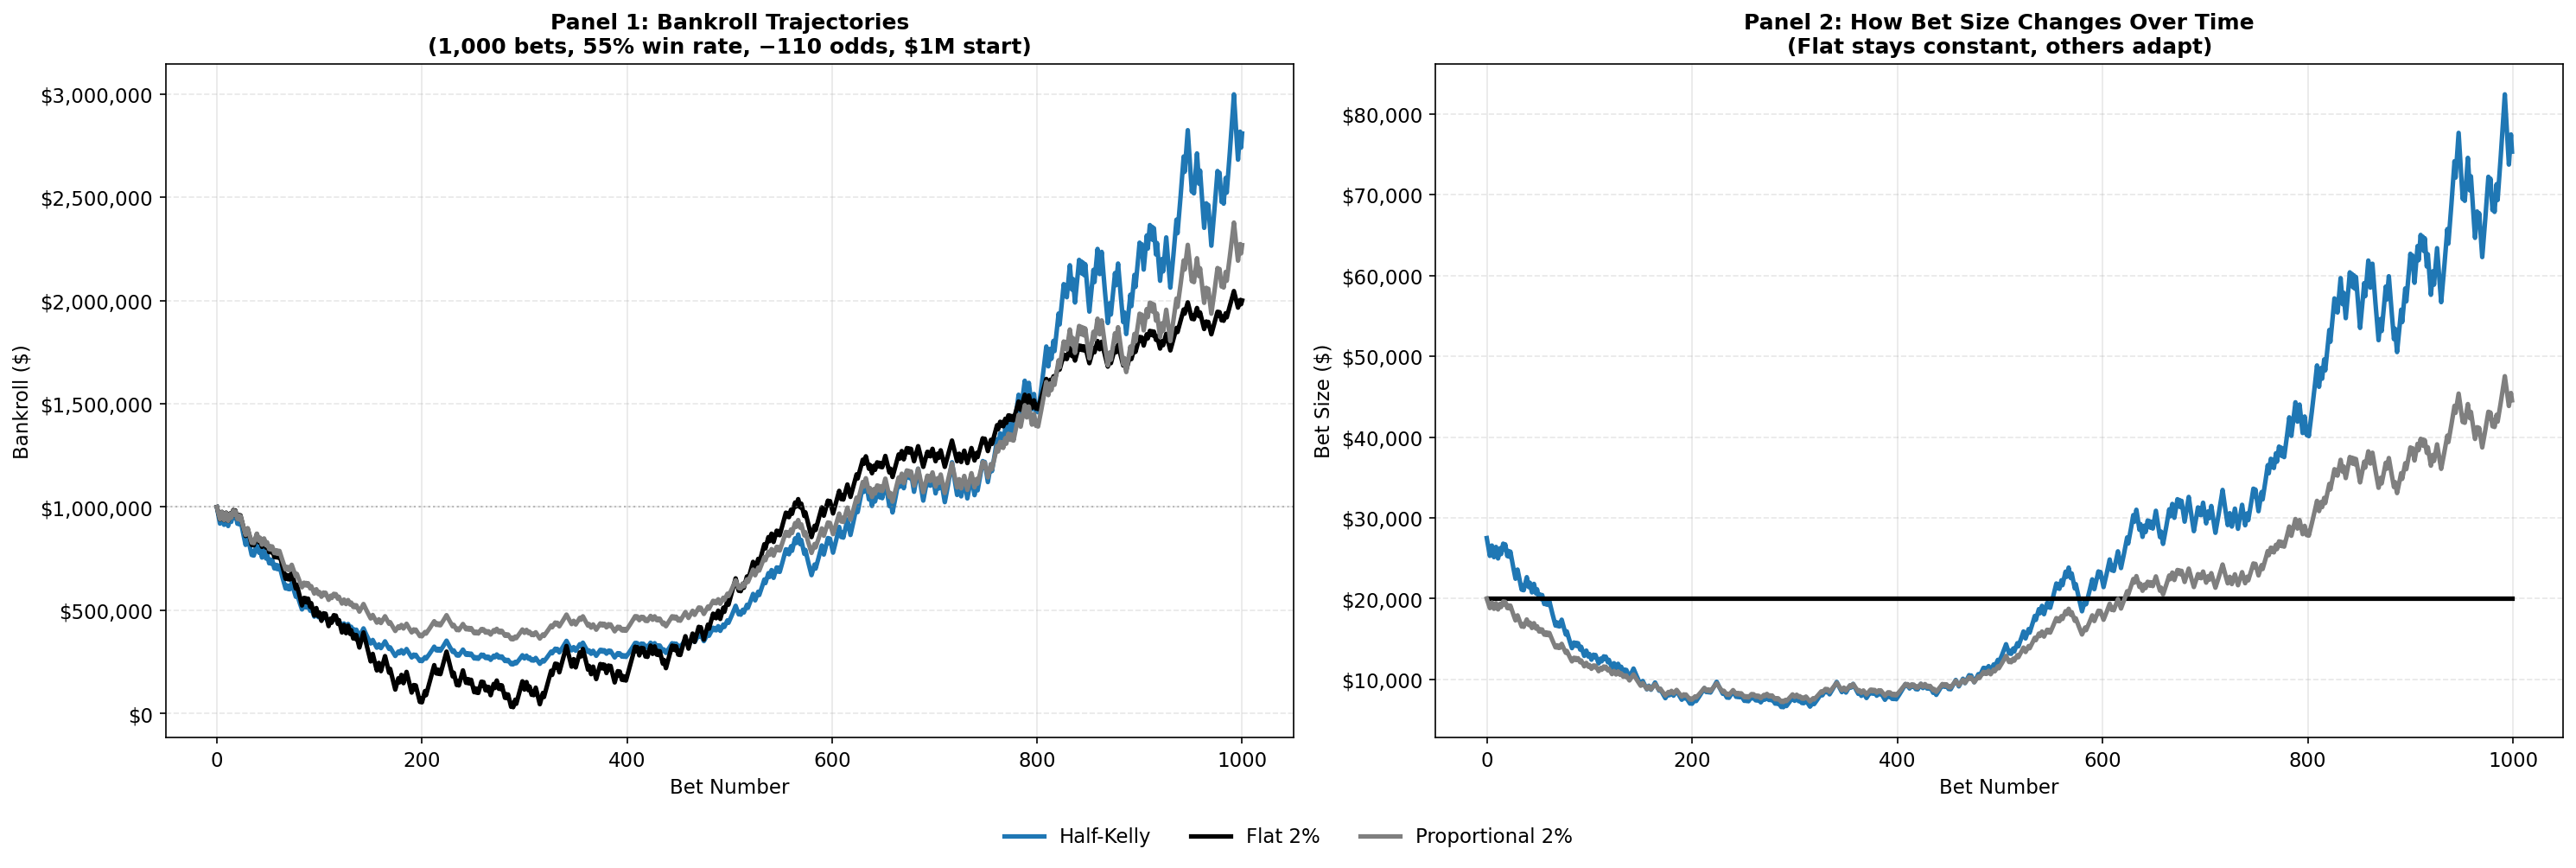
\includegraphics[width=0.90\linewidth]{Images/notitle/nofig11_bet_sizing_explainer.png}
    \caption{Three bet-sizing families on a simulated 1,000-bet sequence at 55\% win rate.}
    \label{fig:11}
\end{figure}

Flat sizing risks bankruptcy when bets exceed the remaining bankroll. Proportional sizing adapts but grows more slowly. Kelly maximises growth but produces extreme volatility when edge estimates are uncertain.

\begin{figure}[H]
    \centering
    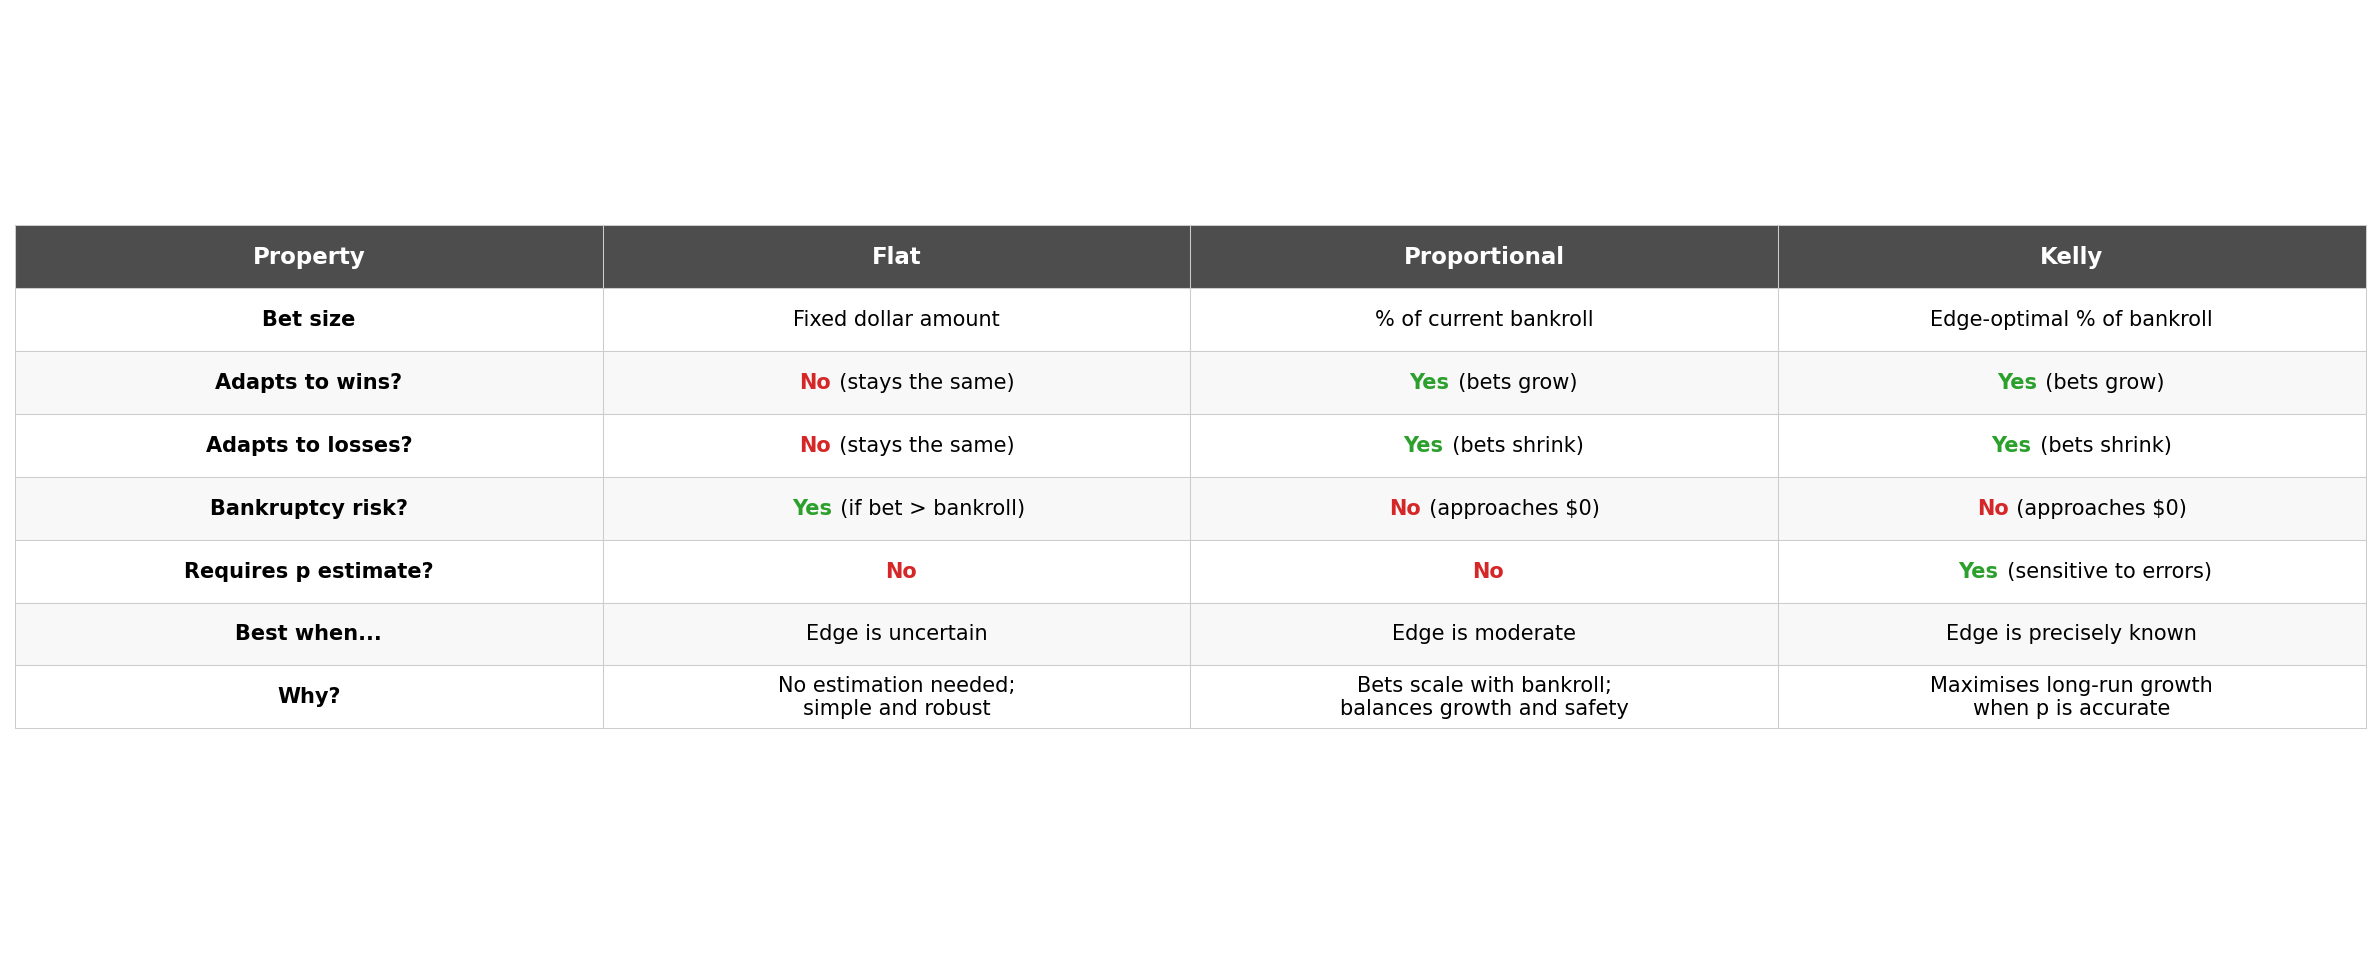
\includegraphics[width=0.55\linewidth]{Images/notitle/nofig12_strategy_properties.png}
    \caption{Structural properties of the three bet-sizing families.}
    \label{fig:12}
\end{figure}

Flat 5\% causes bankruptcy for all four models despite positive edges. Full Kelly achieves the highest CAGR for Ridge ($+10.6\%$) but with 76.6\% max drawdown. For thin-edge models, flat sizing outperforms Kelly because the Kelly fraction (${\sim}1.9\%$) is so small that fixed \$200 bets compound faster.

\begin{figure}[H]
    \centering
    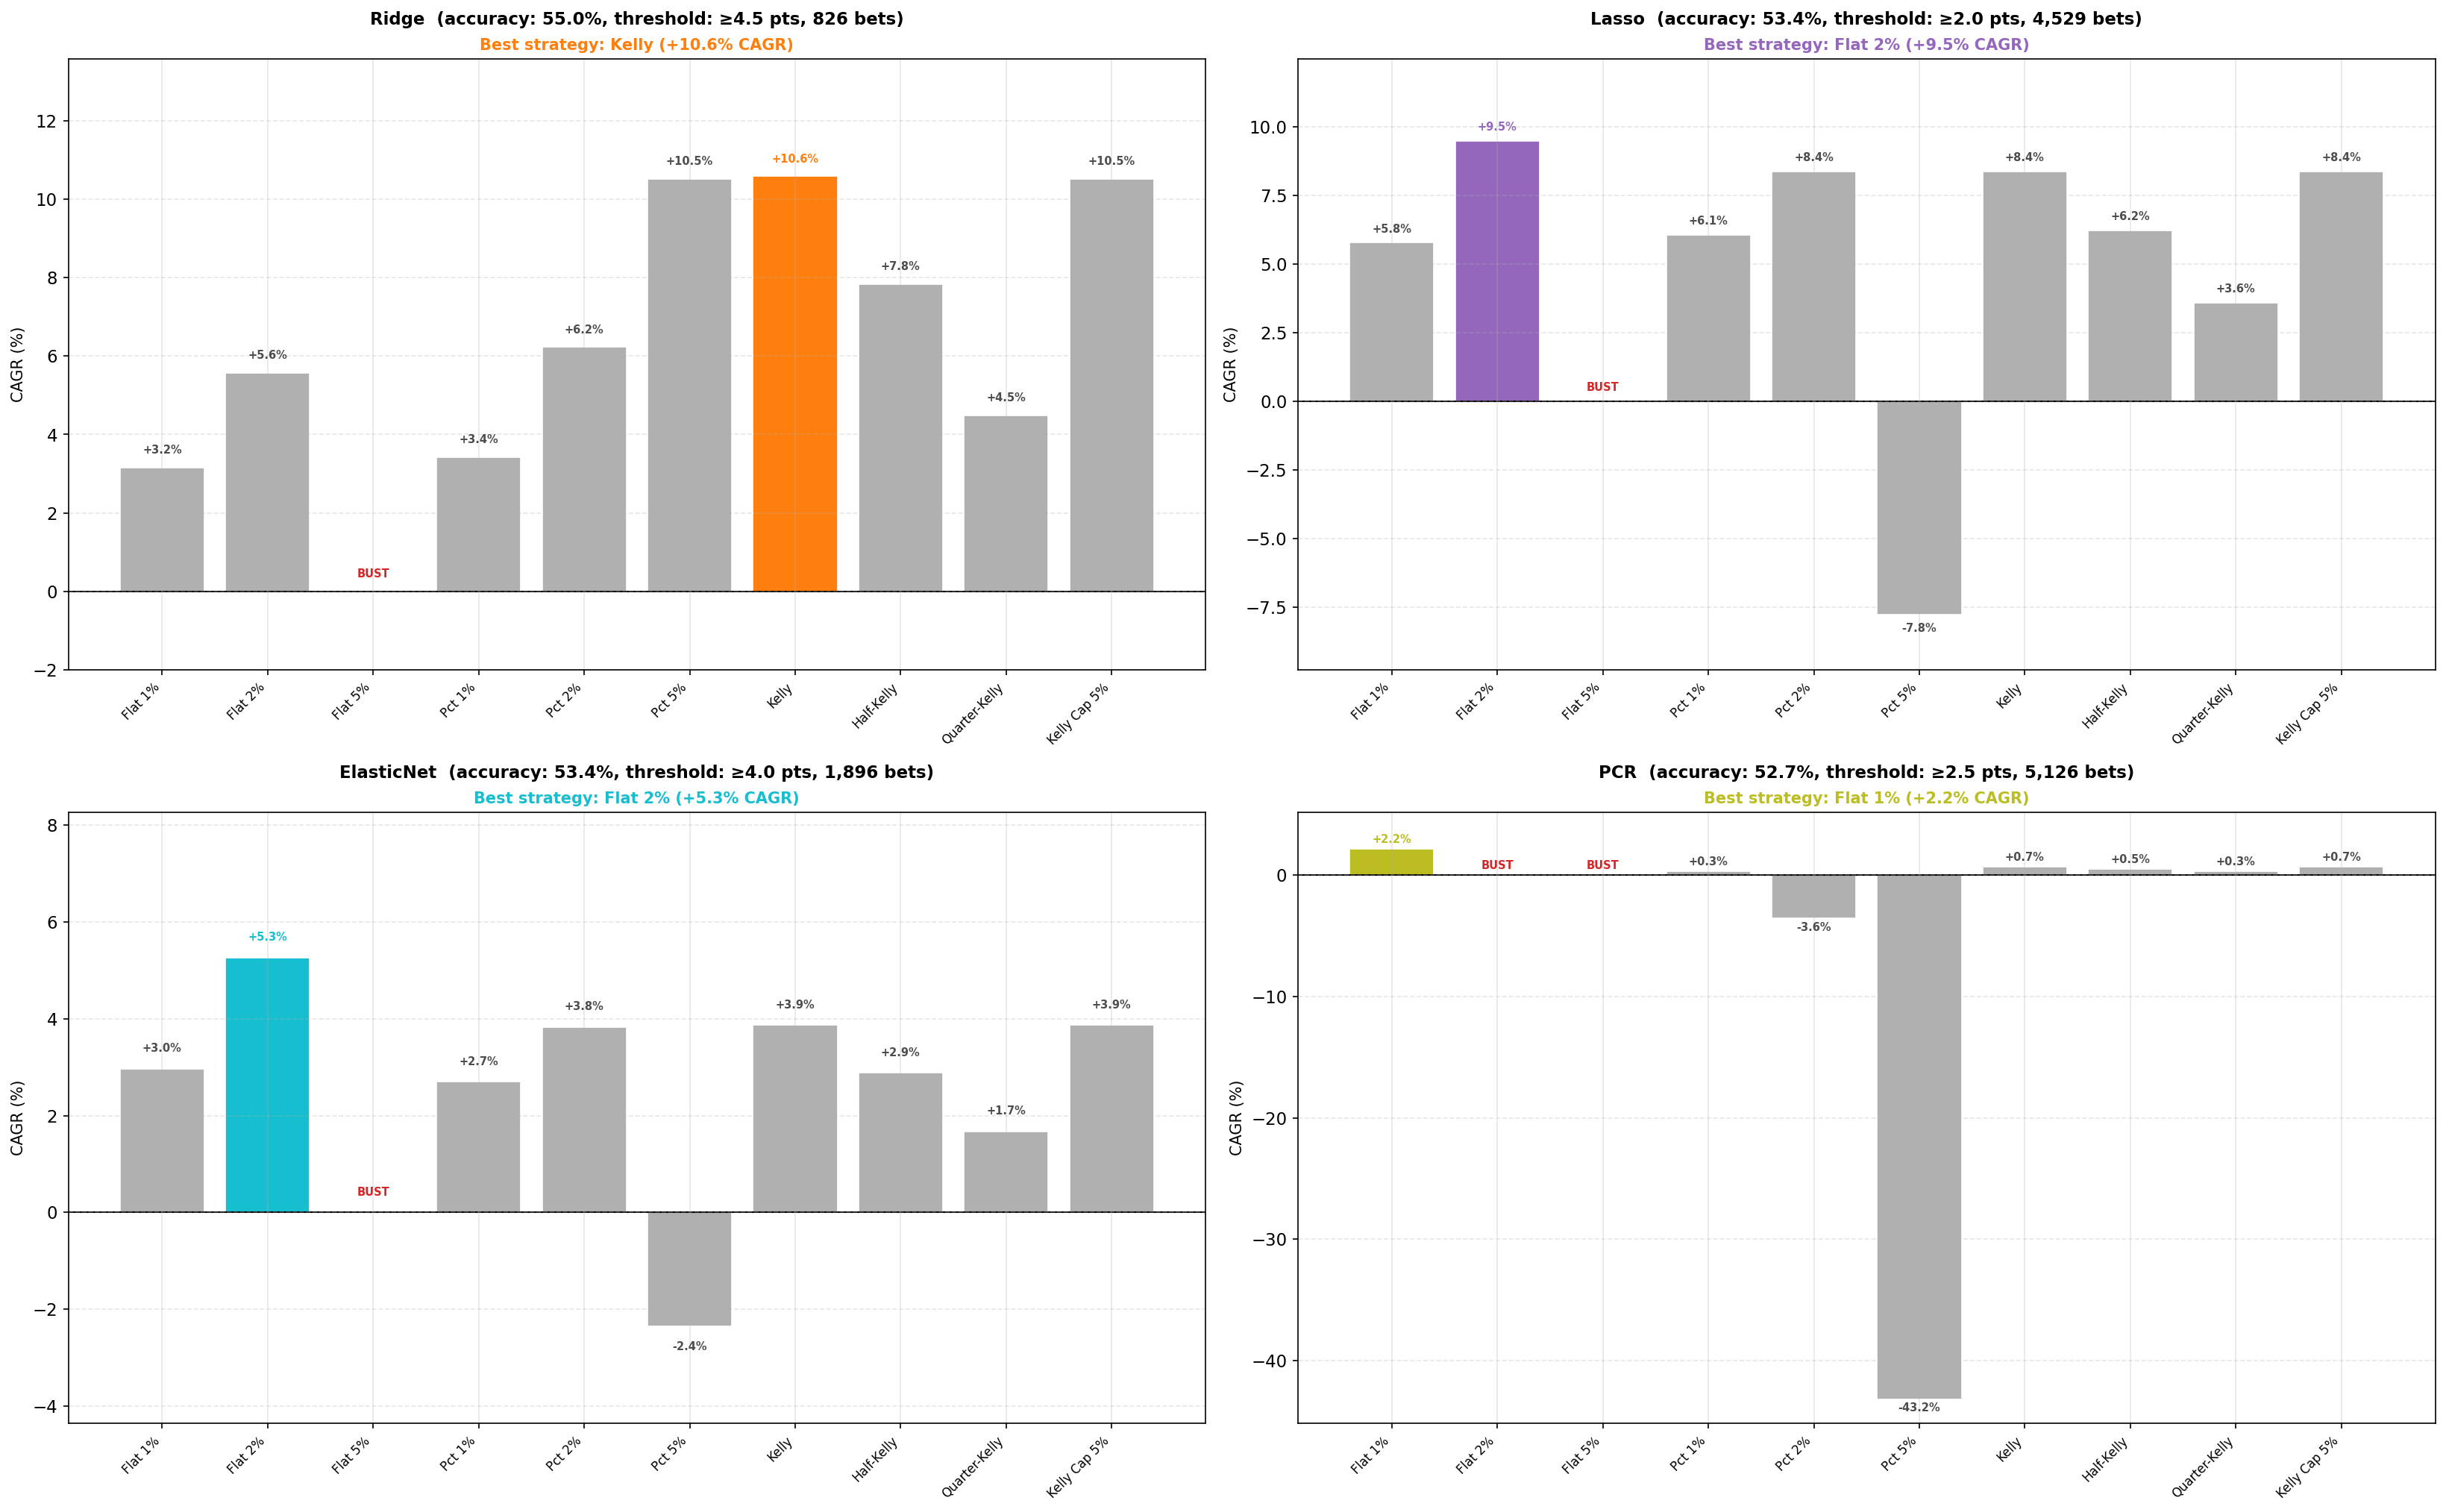
\includegraphics[width=0.90\linewidth]{Images/notitle/nofig13_best_strategy_per_model.png}
    \caption{CAGR across all 10 sizing strategies per model. Best highlighted; bankrupt in red.}
    \label{fig:13}
\end{figure}

\subsection{Model Nomination}
\begin{figure}[H]
    \centering
    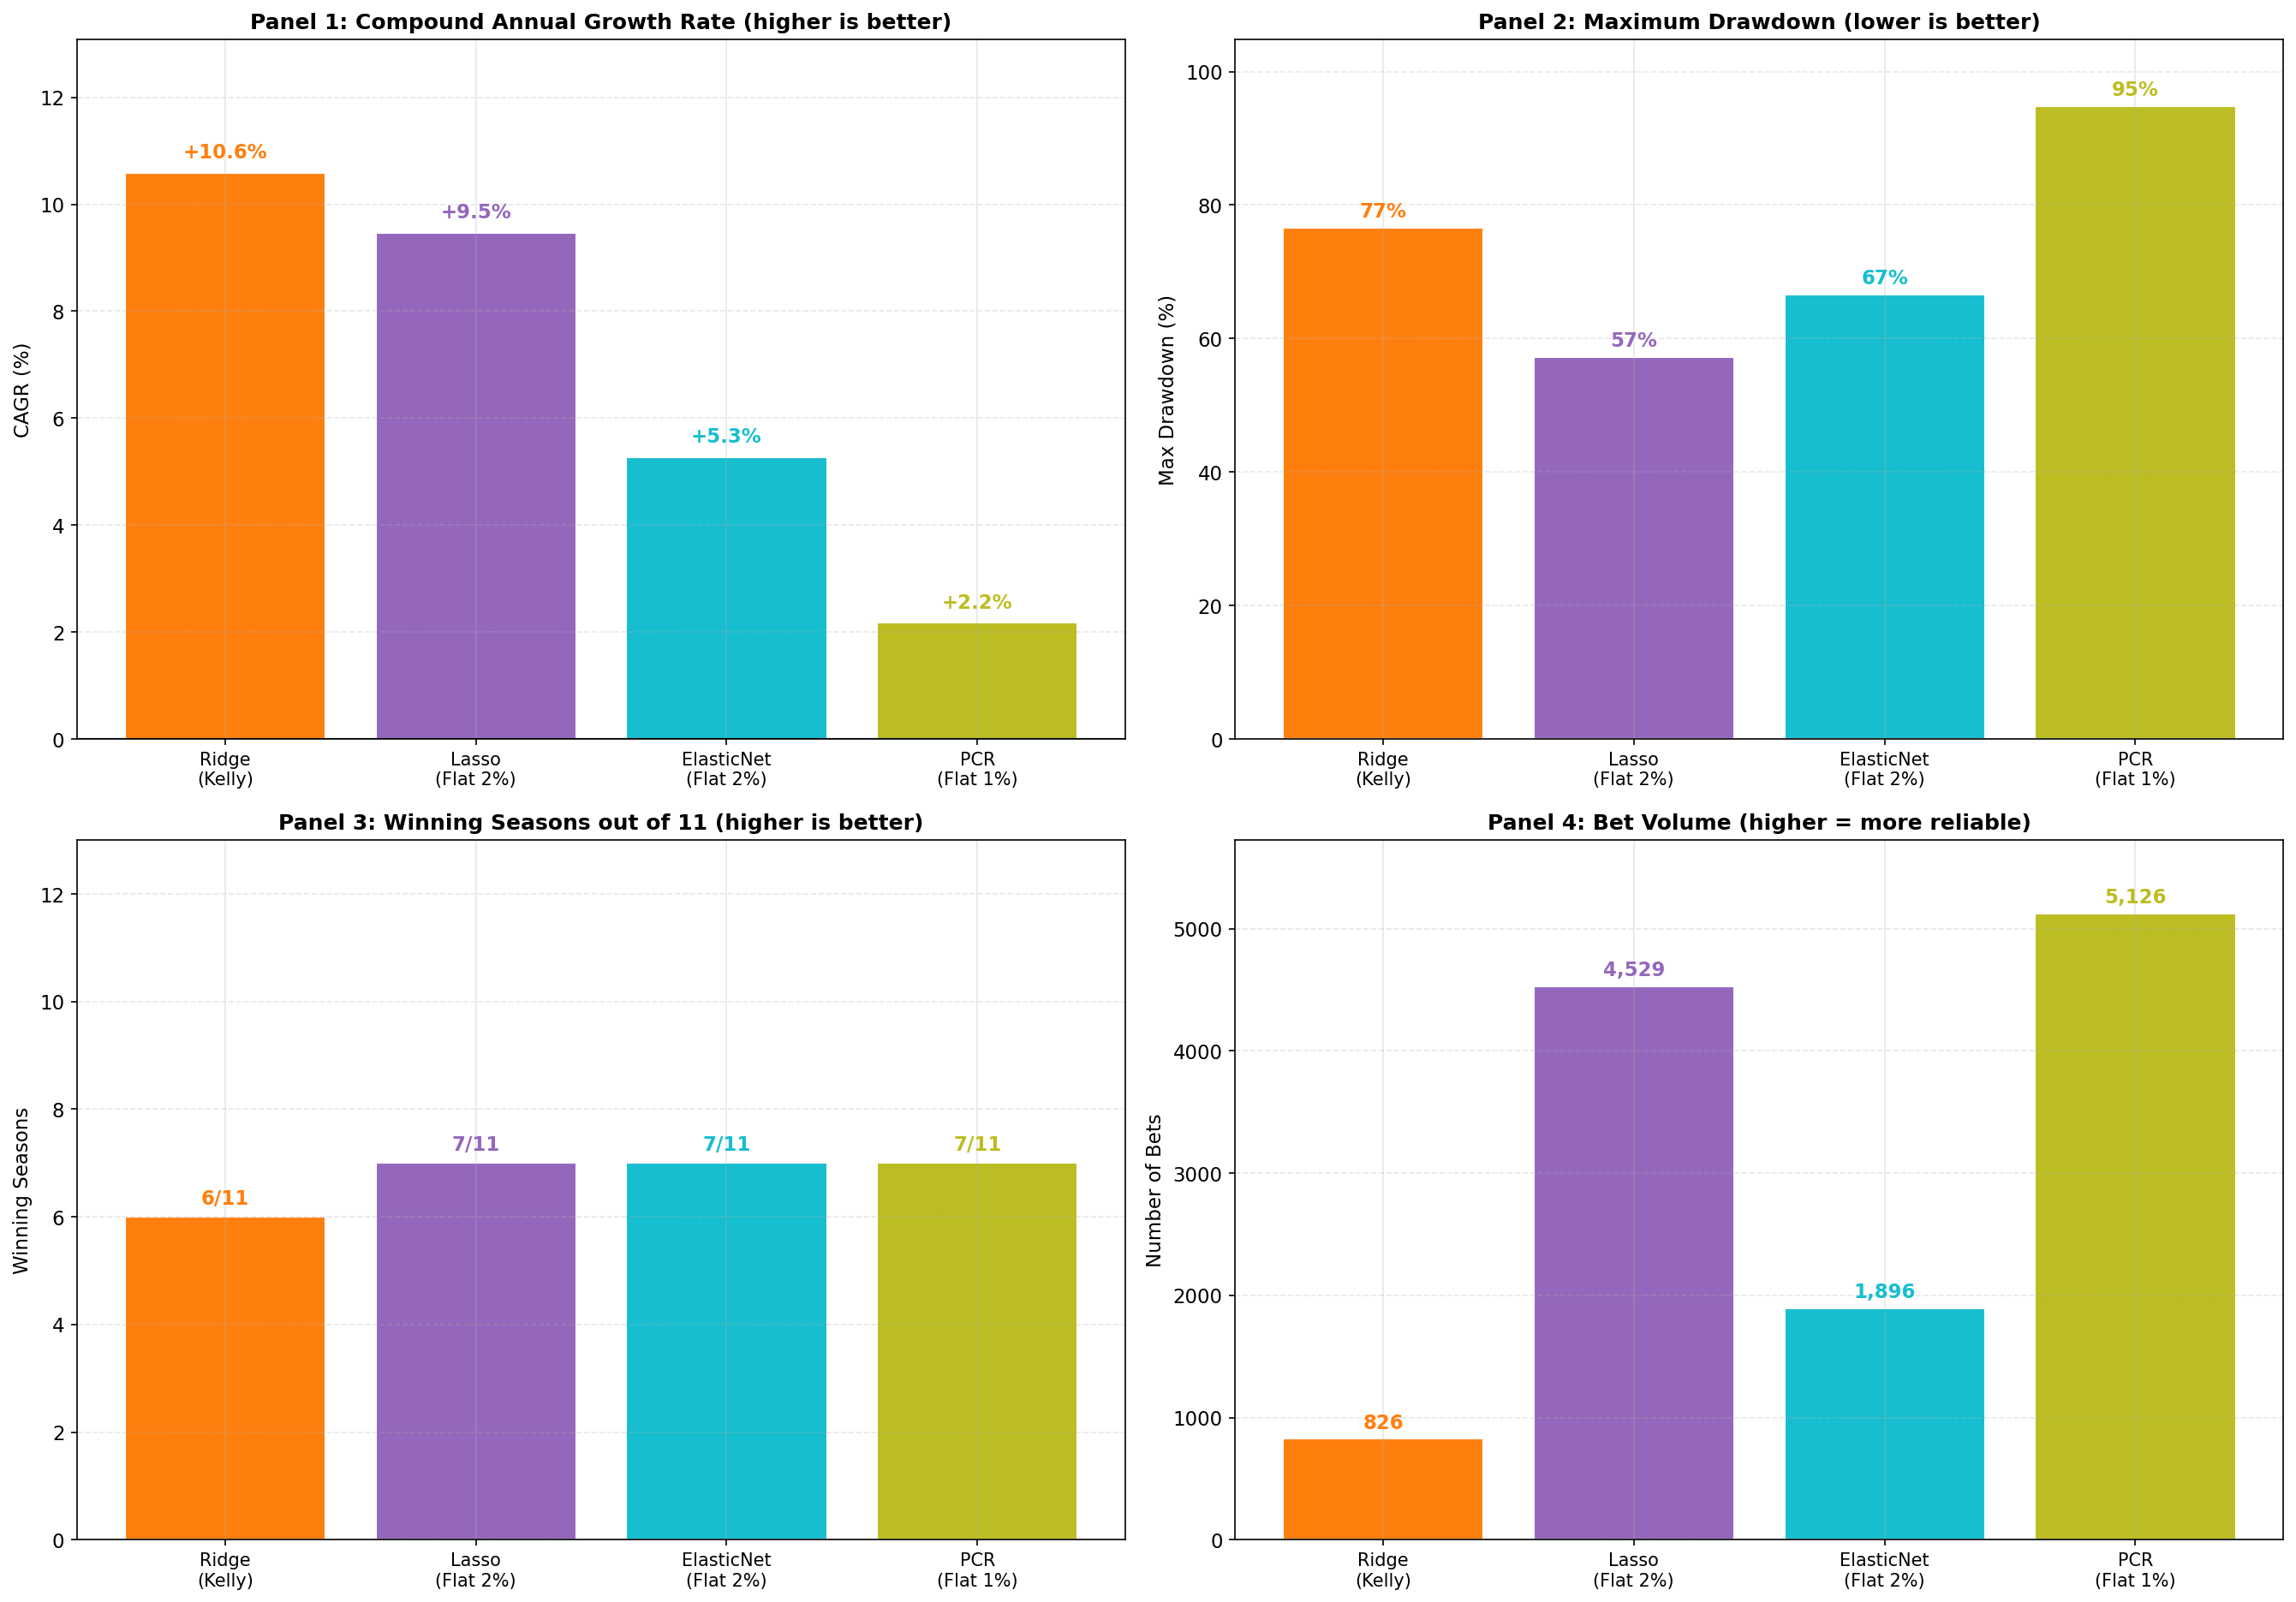
\includegraphics[width=0.90\linewidth]{Images/notitle/nofig14_model_head_to_head.png}
    \caption{Head-to-head comparison: CAGR, max drawdown, winning seasons, bet volume.}
    \label{fig:14}
\end{figure}

Using only pre-2024/25 backtest data, we compare the two leading candidates:

\vspace{-2pt}
\begin{table}[H]
\centering\small
\begin{tabular}{lccc}
\toprule
\textbf{Criterion} & \textbf{Ridge (Kelly)} & \textbf{Lasso (Flat 2\%)} & \textbf{Advantage} \\
\midrule
CAGR & $+10.6\%$ & $+9.5\%$ & Ridge (+1.1pp) \\
Max Drawdown & $76.6\%$ & $57.2\%$ & \textbf{Lasso} \\
Winning Seasons & 6/11 & 7/11 & \textbf{Lasso} \\
Backtest Bets & 826 & 4,529 & \textbf{Lasso} ($5.5\times$) \\
Sizing Complexity & Requires $p$ estimate & Fixed \$200 & \textbf{Lasso} \\
\bottomrule
\end{tabular}
\end{table}
\vspace{-4pt}

We nominate \textbf{Lasso with Flat 2\% sizing (\$200/bet, threshold $\geq 2.0$ points)}. While Ridge offers marginally higher CAGR, Lasso wins on every other dimension: lower drawdown, more winning seasons, $5.5\times$ more bets for statistical reliability, and simpler sizing. This nomination is entirely prospective.

\subsection{Holdout Results: 2024/25 Season}
The Lasso model is retrained on all data through 2023/24. It places 256 qualifying bets on the unseen 2024/25 season, achieving $53.1\%$ accuracy---within $0.3$pp of its 11-season backtest accuracy of $53.4\%$, and above break-even. Under Flat 2\% sizing, the \$10,000 bankroll grows to \$10,727 ($+7.3\%$ return, $15.3\%$ max drawdown).

\begin{figure}[H]
    \centering
    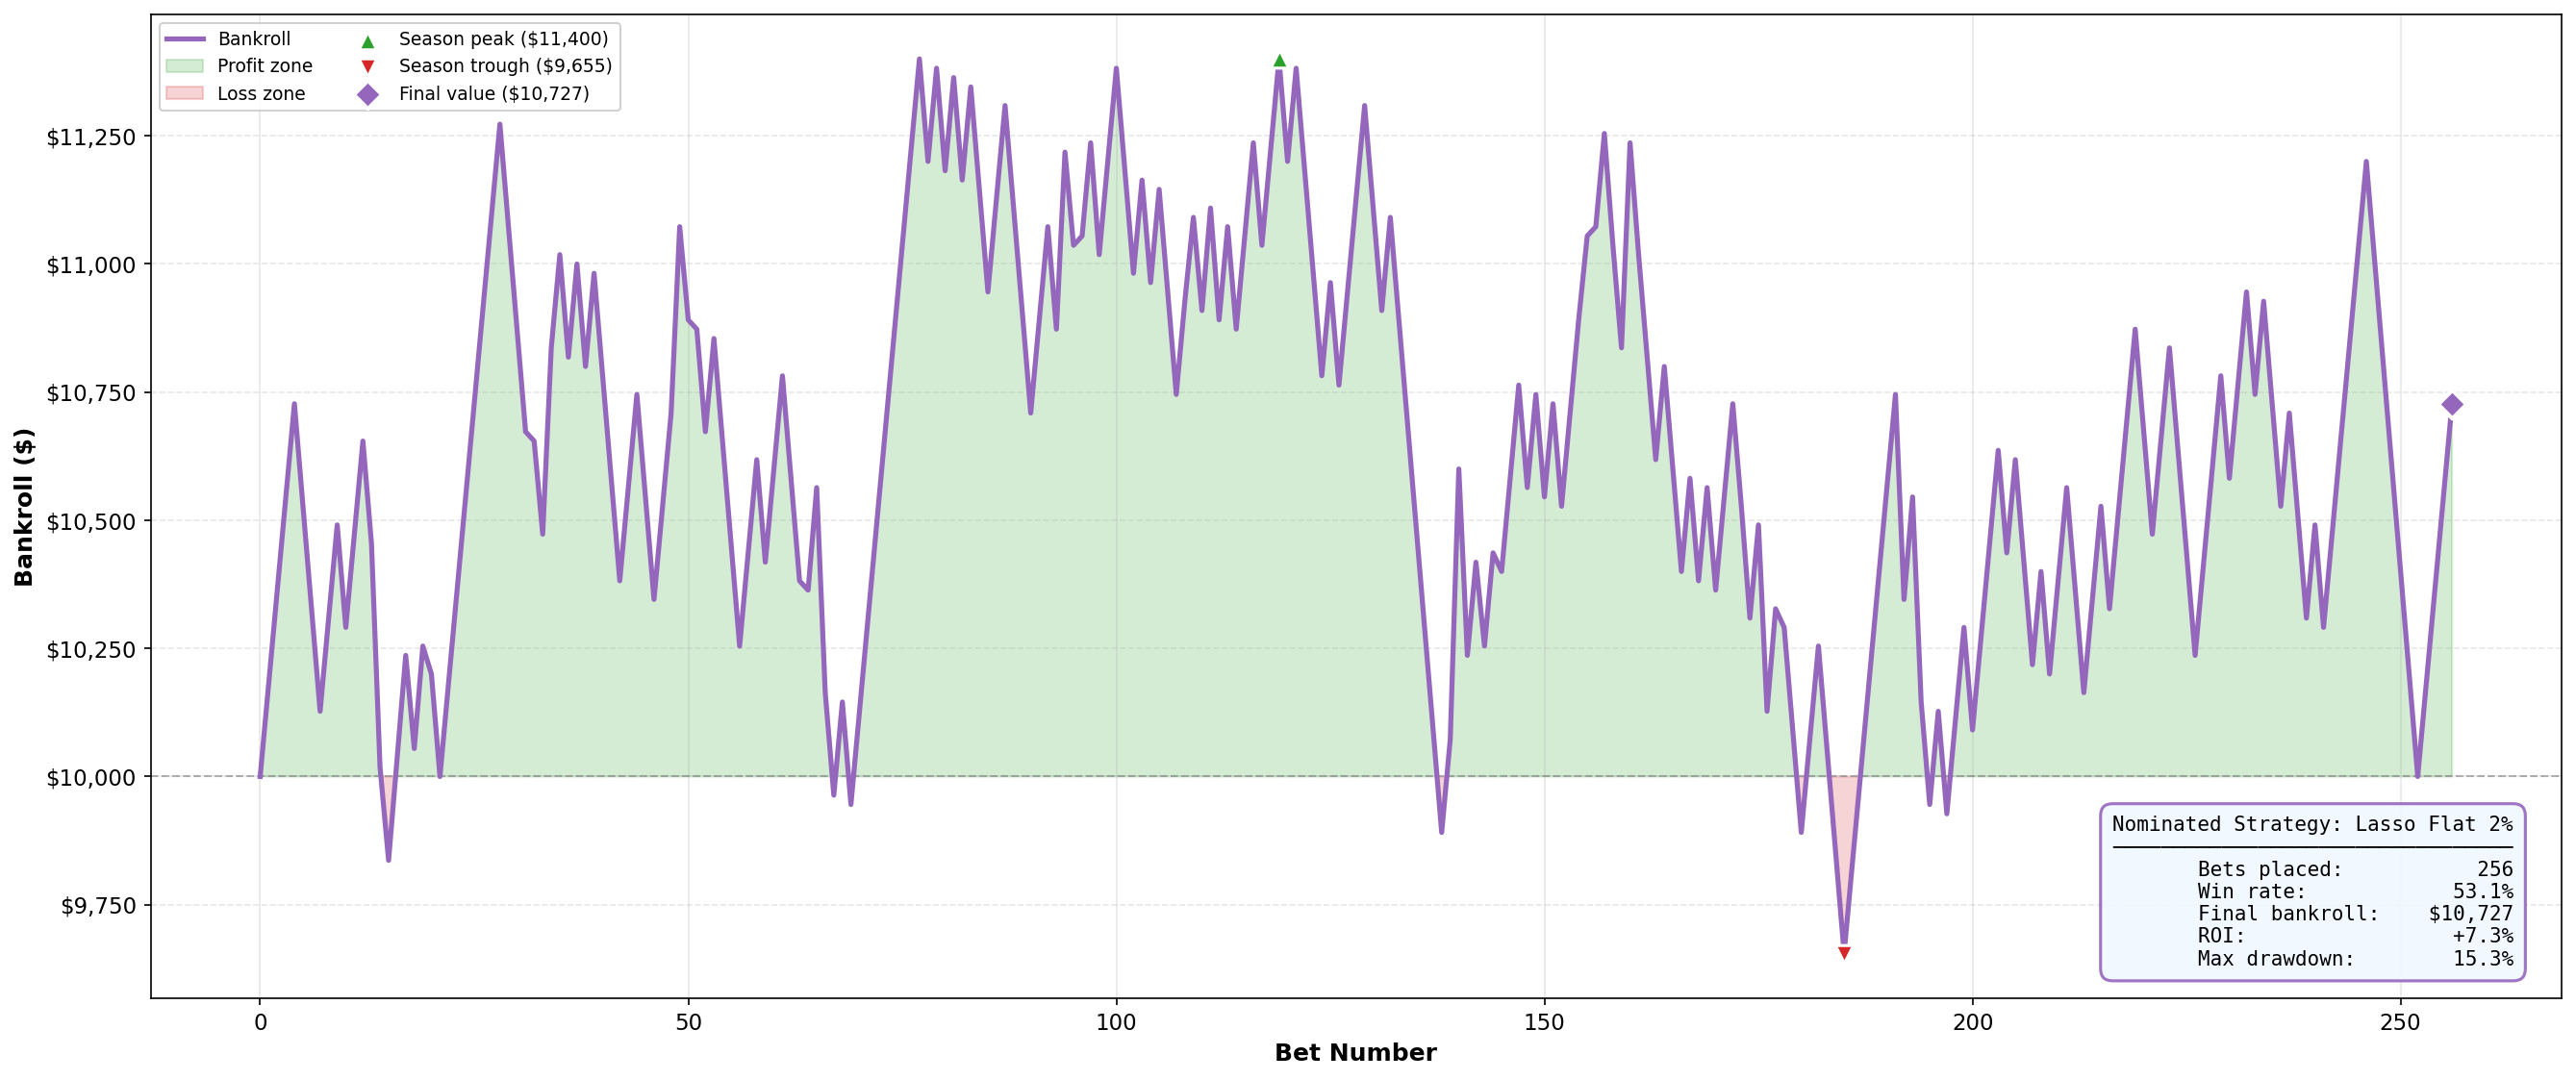
\includegraphics[width=0.90\linewidth]{Images/notitle/nofig15_lasso_holdout_deployment.png}
    \caption{Lasso Flat 2\% bankroll trajectory on the 2024/25 holdout.}
    \label{fig:15}
\end{figure}
\vspace{-4pt}
\begin{figure}[H]
    \centering
    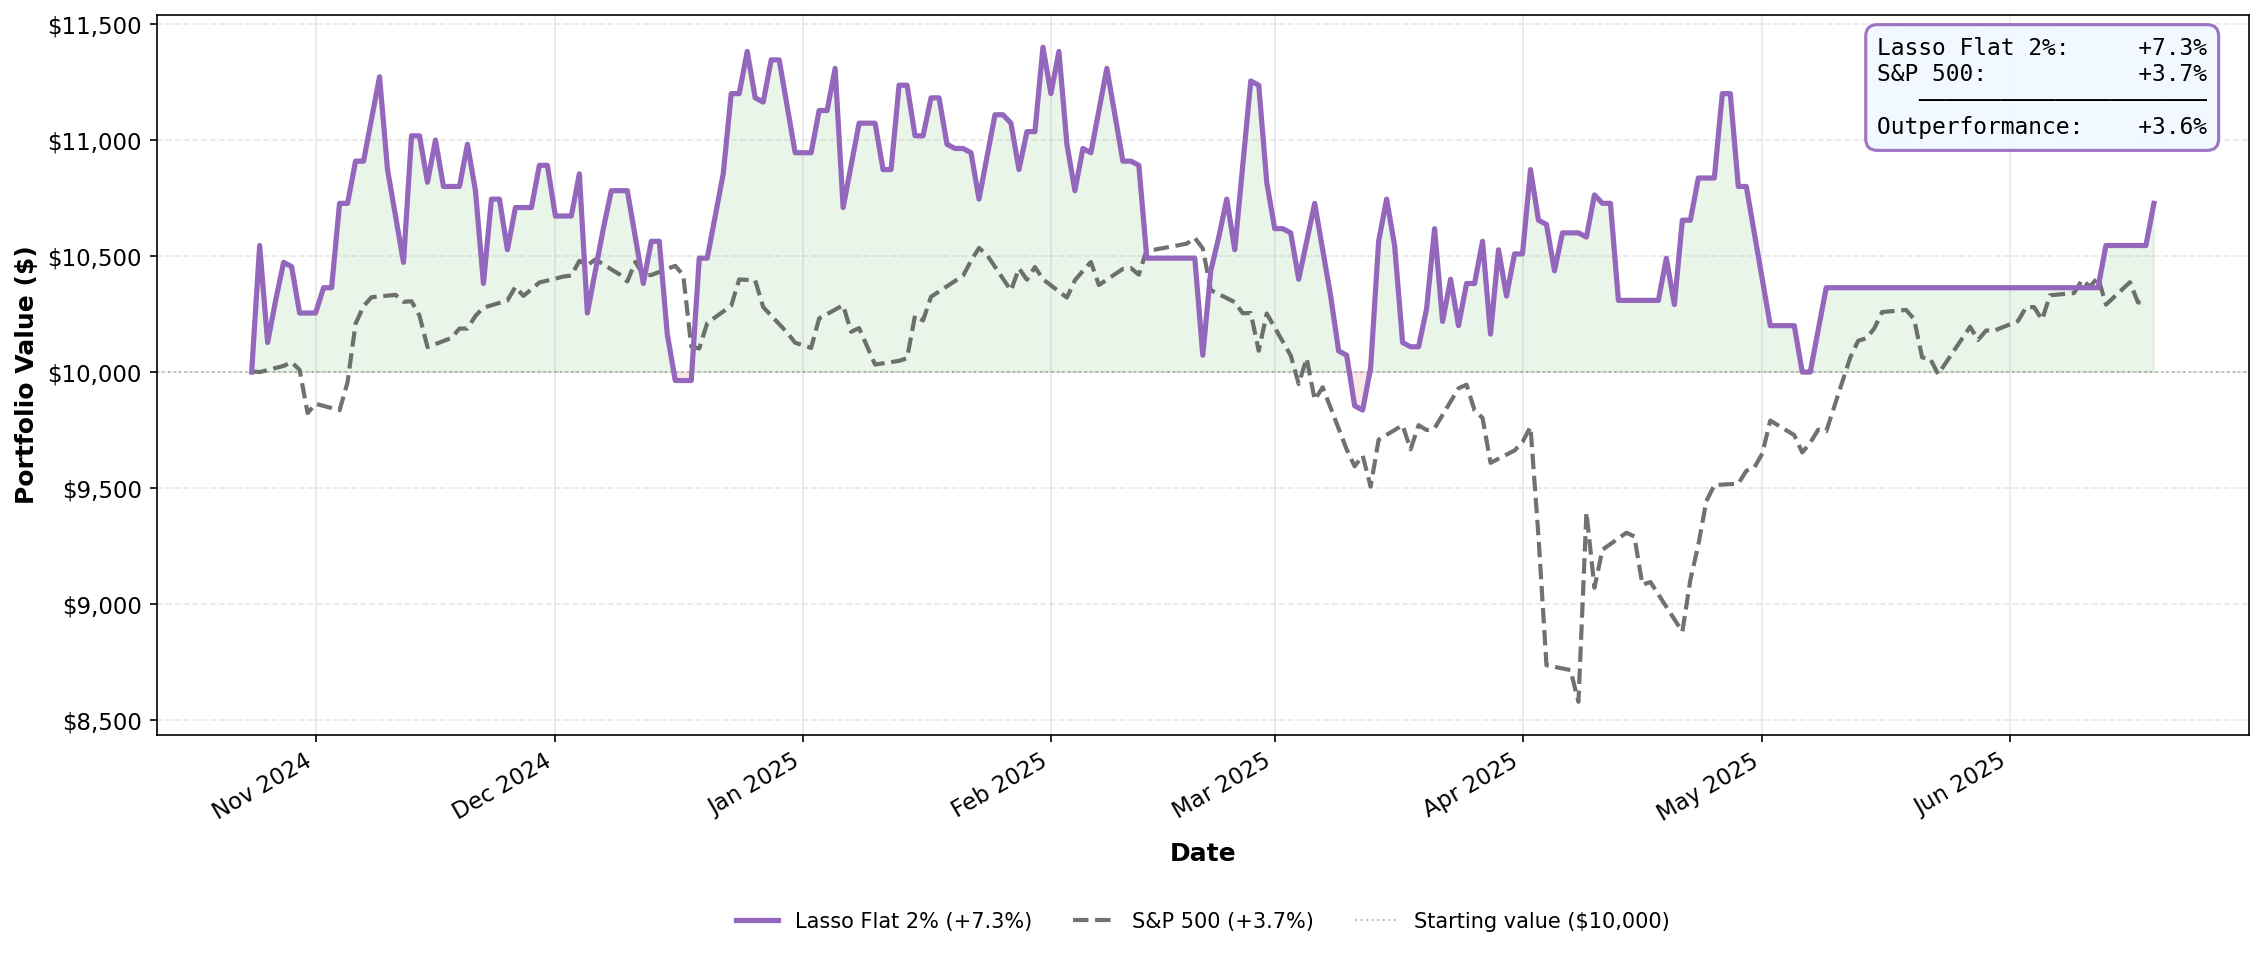
\includegraphics[width=0.90\linewidth]{Images/notitle/nofig16_lasso_vs_sp500.png}
    \caption{Lasso Flat 2\% vs.\ S\&P 500 over the 2024/25 season. Returns are near-zero correlated.}
    \label{fig:16}
\end{figure}

The consistency between backtest and holdout is the most important finding:

\vspace{-2pt}
\begin{table}[H]
\centering\small
\begin{tabular}{lcc}
\toprule
\textbf{Metric} & \textbf{Backtest (11 seasons)} & \textbf{Holdout (2024/25)} \\
\midrule
Accuracy & $53.4\%$ & $53.1\%$ \\
ROI / CAGR & $+9.5\%$ CAGR & $+7.3\%$ ROI \\
Max Drawdown & $57.2\%$ & $15.3\%$ \\
Bet Volume & 4,529 (${\sim}$412/season) & 256 \\
\bottomrule
\end{tabular}
\end{table}
\vspace{-4pt}

The strategy's $+7.3\%$ return compares to the S\&P~500's $+3.7\%$ over the same period, with near-zero correlation to equity markets (Figure~\ref{fig:16})---a diversification benefit independent of traditional asset classes. However, 256 bets is statistically underpowered: the 95\% Wilson CI spans $[47.0\%, 59.1\%]$, including both $50\%$ and $52.4\%$. The mild holdout drawdown is well below the backtest worst case; future seasons could be harsher. The key finding is directional consistency: the edge did not disappear on new data.

%% =====================================================================
%%  SECTION 8: REAL-WORLD IMPLEMENTATION CONSTRAINTS
%% =====================================================================
\section{Real-World Implementation Constraints}
Three frictions---analogous to transaction costs, liquidity limits, and market impact---stand between a profitable backtest and actual profit.

\textbf{Execution slippage.} Slippage is the difference between the line when we \emph{identify} a bet and when we \emph{execute}. Lines move continuously in response to sharp money and sportsbook algorithms that detect one-sided action. Because our model targets line mispricings using public data, the same information flow that creates our edge drives adverse line movement. Crucially, this movement is predominantly \emph{adversarial}: lines move toward the true value, which is the same direction as our bet, so slippage almost always works against model-based bettors. For a strategy whose holdout edge is just 0.7pp above break-even---roughly 7 extra wins per 1,000 bets---typical NBA line movement of 0.5--1.5 points is an existential threat. Many of our winning bets are decided by narrow margins; even a half-point line shift can flip some narrow wins into losses. A rigorous analysis would model slippage as a stochastic process with per-bet draws from a distribution of line movements, but the qualitative conclusion is robust: a sub-one-percentage-point edge cannot tolerate whole-point line movements.

\textbf{Market depth and scalability.} Sportsbooks impose per-game limits of \$5,000--\$10,000 on NBA totals. Across ${\sim}$10 legal US books, the aggregate ceiling is ${\sim}$\$2.5--5M under Flat 2\% sizing, but multi-book execution requires near-instantaneous infrastructure, sportsbooks share sharp-bettor intelligence, and large one-directional bets create self-induced slippage. The strategy works best at small scale.

\textbf{Account restrictions.} Sportsbooks track \emph{Closing Line Value} (CLV)---whether a bettor consistently receives better odds than the closing line. Persistent positive CLV triggers restrictions: reduced limits (sometimes to \$1/bet), account closure, or delayed bet acceptance. Profitable accounts are typically flagged within 1--3 seasons. Our Lasso strategy, which targets line mispricings by design, would exhibit exactly the CLV pattern that triggers restrictions---imposing a hard time limit regardless of whether the edge persists.

%% =====================================================================
%%  SECTION 9: CONCLUSION
%% =====================================================================
\section{Conclusion}
This project set out to determine whether ML models can profitably predict NBA over/under totals. The answer is nuanced: a genuine statistical edge exists, but real-world frictions make it extremely difficult to capture.

\textbf{The edge is real.} Linear models achieve $51.7$--$52.0\%$ accuracy on $>$14,000 OOS predictions ($p < 0.001$ after Bonferroni). Selective betting pushes four models above $52.4\%$, with Ridge at $55.0\%$ and $+5.4\%$ ROI.

\textbf{Simple models dominate.} XGBoost's 2.3-point train-vs-OOS RMSE gap confirms memorisation. In an efficient market, model flexibility is a liability---a textbook bias-variance tradeoff.

\textbf{The holdout confirms the backtest.} Lasso Flat 2\% achieved $53.1\%$ accuracy on 256 unseen bets ($+7.3\%$ return), with near-zero equity-market correlation. This consistency is the project's most important result, though one season is insufficient for certainty.

\textbf{Real-world viability is limited.} Slippage of 0.5--1.5 points threatens a $<$1pp edge, betting limits constrain scale, and account restrictions impose a 1--3 season horizon.

\textbf{Market efficiency.} The NBA over/under market is efficient in the practical sense: publicly available information is largely priced into the Vegas line, and the residual inefficiency is small enough that transaction costs and structural constraints prevent reliable capture. As an academic exercise, the Lasso strategy demonstrates that machine learning can extract signal from NBA game data slightly beyond what the Vegas line reflects. As a practical investment, it would require near-perfect execution, access to multiple high-limit accounts, and a willingness to accept a 1--3 season lifespan. The gap between statistical and economic significance is the defining challenge of applied machine learning in efficient markets.

\end{document}
